  \documentclass[12pt, a4paper]{article}

  % ── Packages ─────────────────────────────────────────────────────────────────
  \usepackage[a4paper, margin=2.5cm]{geometry}
  \usepackage{amsmath, amssymb, amsfonts}
  \usepackage{graphicx}
  \graphicspath{{figures/}}
  \usepackage{booktabs}          % professional tables
  \usepackage{array}
  \usepackage{hyperref}
  \usepackage{xcolor}
  \usepackage{caption}
  \usepackage{subcaption}
  \usepackage{natbib}            % bibliography
  \usepackage{setspace}
  \usepackage{fancyhdr}
  \usepackage{titlesec}
  \usepackage{parskip}
  \usepackage{microtype}
  \usepackage{float}
  \usepackage[utf8]{inputenc}
  \usepackage[T1]{fontenc}

  % ── Page style ───────────────────────────────────────────────────────────────
  \onehalfspacing
  \pagestyle{fancy}
  \fancyhf{}
  \rhead{\small Multi-Agent AIS Trajectory Prediction}
  \lhead{\small Aviv Salomon}
  \cfoot{\thepage}
  \setlength{\headheight}{14pt}

  % ── Helpers ──────────────────────────────────────────────────────────────────
  \newcommand{\TODO}[1]{\textcolor{red}{\textbf{[TODO: #1]}}}
  \newcommand{\FILL}[1]{\textcolor{blue}{\textbf{[FILL: #1]}}}

  % ─────────────────────────────────────────────────────────────────────────────
  \begin{document}

  % ── Title page ───────────────────────────────────────────────────────────────
  \begin{titlepage}
      \centering
      \vspace*{1cm}

      {\large School of Software Engineering: MSc Intelligent Systems}\\[0.5cm]
      {\large Final Project Report}\\[1.5cm]

      {\Huge\bfseries Multi-Agent Social Interaction AIS\\[0.3cm]
      Trajectory Prediction:\\[0.3cm]
      Comparing Methods}\\[2cm]

      \begin{tabular}{rl}
          \textbf{Student:}    & Aviv Salomon \\[0.3cm]
          \textbf{Supervisor:} & Dr.\ Sharon Yalov-Handzel \\
                               & Head of the Master's Program, \\
                               & School of Software Engineering \\[0.3cm]
          \textbf{Advisor:}    & Mr.\ Anton (Yurkov) Feingold \\
                               & AI Team Lead, Orca AI \\[0.3cm]
          \textbf{Date:}       & October 2026 \\
      \end{tabular}

      \vfill
  \end{titlepage}

  % ── Abstract ─────────────────────────────────────────────────────────────────
  \begin{abstract}
Vessel trajectory prediction from AIS underpins automated collision avoidance,
  yet published results in this field cannot be compared with one another: each
  study reports on a private regional dataset, at its own prediction horizon,
  under its own preprocessing and metric conventions.  We address this by
  evaluating five architectures under a single protocol --- an ordinary
  least-squares baseline, TrAISformer, AIS-ACNet, GAT-LSTM, and Wayformer-AIS, a
  maritime adaptation of a multi-agent attention model --- on the same corpus of
  operational AIS, at a common five-minute horizon sampled at 1\,Hz, with
  identical splits and metric implementations and a held-out test set of
  11{,}891 prediction windows.

  The comparison produces a result the maritime literature does not currently
  surface: at this horizon three of the four learned architectures predict less
  accurately than constant-velocity extrapolation of the observed track.  Only Wayformer-AIS
  improves on that baseline, reaching 15.57\,m minADE$_6$ and 31.71\,m
  minFDE$_6$ against 26.70\,m and 51.43\,m, and its margin widens as manoeuvre
  difficulty rises --- from 3.2\,m on stationary vessels to 49.5\,m on sharp
  turns.  It is also the only model in the comparison given the surrounding
  traffic as input rather than a single vessel's track.  Stratified analysis
  locates the remaining error in underway vessels in dense traffic and in turns
  already in progress.  The preprocessing pipeline, model configurations and
  evaluation scripts are released so that the comparison can be repeated and
  extended.
  \end{abstract}

  \newpage
  \tableofcontents
  \newpage

  % ─────────────────────────────────────────────────────────────────────────────
  \section{Introduction}
  \label{sec:intro}

  \subsection{Motivation}

  The global maritime sector carries more than 80\,\% of world trade by volume, and vessel
  traffic continues to grow alongside expanding global supply chains.  As ships become larger
  and operating margins tighter, there is mounting demand for autonomous and decision-support
  systems capable of reducing human error, improving situational awareness, and enforcing
  compliance with the International Regulations for Preventing Collisions at Sea
  (COLREGs)~\citep{colregs1972}.

  At the core of any autonomous maritime system lies a classical autonomy pipeline:
  \textit{perception} (detecting other vessels from radar, camera, or AIS),
  \textit{prediction} (estimating where those vessels will be in the near future), and
  \textit{planning} (computing a safe, COLREG-compliant manoeuvre for the ego vessel).
  Trajectory prediction is the bridge between perception and planning: a collision-avoidance
  planner cannot reason about a safe path without a probabilistic estimate of how nearby
  vessels will move~\citep{kuwata2014safe, vagale2021path, mahipala2025colreg}.
  Constant-velocity assumptions, the default fallback in many deployed systems, break down
  precisely in the situations that matter most --- congested ports, narrow channels, and
  overtaking or crossing encounters governed by COLREG rules.  Accurate, interaction-aware
  trajectory prediction is therefore not an academic exercise but a safety-critical
  prerequisite for practical autonomous bridge deployment.

  The Automatic Identification System (AIS) provides the natural data foundation for
  this prediction task~\citep{itu2014ais}.  Under IMO mandate, every large commercial
  vessel continuously broadcasts its MMSI, position, speed, and course at intervals as
  short as 2\,seconds, producing a dense, global, and freely receivable record of maritime
  motion.  The richness of this signal has driven a wave of data-driven trajectory
  prediction research over the past decade, spanning recurrent networks, graph models,
  and transformers (see Section~\ref{sec:related}).

  This study is motivated in part by the operational context of Orca AI, a company that
  deploys AI-based situational awareness systems on commercial vessels worldwide.
  Orca AI's onboard AIS integration produces a large-scale, geographically diverse
  archive of real maritime encounters accumulated since 2019, offering an opportunity
  to train and evaluate prediction models on operational data of a kind not commonly
  available to academic research.  The corpus used in this work is a subset of that
  archive.
  Crucially, the scenarios in this dataset are captured from the perspective of a navigating
  vessel (\textit{ego vessel}) surrounded by up to tens of nearby \textit{target vessels},
  making the interaction structure --- which vessel is on a collision course, which is merely
  passing --- an integral part of the prediction problem.

  \subsection{The Comparison Problem in Maritime AI}

  Despite a growing body of AIS prediction literature, a practitioner seeking to select
  or deploy a model faces a fundamental obstacle: the published results cannot be
  meaningfully compared.  TrAISformer~\citep{nguyen2021traisformer} is evaluated on
  Finnish–Baltic AIS data with a 30-minute horizon and cross-entropy loss;
  AIS-ACNet~\citep{shin2024aisacnet} uses South Korean coastal data with 10-second
  prediction steps; GAT-LSTM~\citep{zhao2023gatlstm} reports next-step ADE on
  Chinese coastal waters; TPTrans~\citep{wang2024tptrans} evaluates on a Chinese
  port dataset with its own normalisation scheme.  Each paper applies its own
  preprocessing, defines its own evaluation horizon, and reports on a proprietary
  regional dataset that no other group can access.

  The consequence is that the basic question --- \textit{does a transformer outperform a
  graph network for vessel trajectory prediction, and by how much?} --- cannot be answered
  from the existing literature.  Method comparisons within individual papers are invariably
  partial, comparing only against baselines the authors chose to re-implement, on their
  own data, under their own evaluation protocol.

  This paper resolves the comparison problem by subjecting five architectures --- from a
  na\"{i}ve linear baseline to a multi-agent transformer --- to an identical experimental
  protocol: the same proprietary AIS dataset, the same preprocessing pipeline, the same
  train/validation/test split, and the same evaluation metrics.  The result is the first
  controlled, apples-to-apples comparison of maritime trajectory prediction methods on
  a large-scale, multi-year, globally diverse dataset.

  \subsection{Problem Statement}

  We consider a maritime scene in which several vessels manoeuvre simultaneously
  within mutual observation range, and ask how each of them will move over the
  following minutes.  The input is the recent motion history of every vessel in
  the scene, reconstructed from AIS.  The required output is not a single future
  track per vessel but a small set of plausible alternatives with associated
  probabilities, because a vessel approaching a waypoint or an encounter may
  legitimately hold its course, alter to port or starboard, or slow to a stop.
  Predictions are made independently for each vessel while conditioning on the
  observed histories of all its neighbours, so that interaction informs the
  forecast without requiring the model to commit to a single joint future for
  the whole scene.  Accuracy is judged by how closely the best of the proposed
  alternatives matches what the vessel actually did.

  Section~\ref{sec:problem} states this task formally, together with the input
  and output representations, the observation and prediction horizons, and the
  evaluation metrics used throughout the paper.

  \subsection{Contributions}
  This paper makes the following contributions:
  \begin{enumerate}
      \item \textbf{AIS data pipeline:} A complete pre\-processing toolkit for raw
      AIS CSV data, including de\-duplication, gap interpolation, coordinate
      projection, and UniTraj-com\-pat\-i\-ble serialization.

      \item \textbf{Unified maritime benchmark:} The first evaluation of multiple trajectory
      prediction architectures under identical conditions --- shared train/validation/test splits,
      preprocessing, and metrics --- on a large-scale proprietary AIS dataset.

      \item \textbf{Method comparison:} Systematic evaluation of five approaches ---
      a na\"{i}ve OLS linear baseline, TrAISformer, AIS-ACNet,
      Wayformer-AIS, and GAT-LSTM~\citep{zhao2023gatlstm} --- each adapted to
      and evaluated under identical conditions on the same maritime AIS dataset.

      \item \textbf{Reproducibility:} All code, configuration, and evaluation scripts
      are released to enable future comparisons on the same or alternative AIS datasets.
  \end{enumerate}

  % ─────────────────────────────────────────────────────────────────────────────
  \section{Related Work}
  \label{sec:related}

  Table~\ref{tab:related_work} lists the twelve works reviewed in this section.
  Its purpose is not to summarise their methods --- each is discussed individually
  in the subsections that follow --- but to make a single observation visible at a
  glance: \emph{no two of these studies are evaluated under the same conditions}.
  Each maritime entry reports on a different regional dataset, at a different
  prediction horizon, under its own preprocessing and metric conventions, and
  several do not specify their evaluation setting in reproducible detail at all.
  The absence of any shared row in the final column is precisely the gap this
  paper addresses.

  \begin{table}[H]
    \centering
    \small
    \caption{Related work, with the evaluation setting each study reports.
             $\dagger$ = maritime / AIS domain; unmarked methods originate from
             road-vehicle or pedestrian prediction and are adapted or compared
             in this work.  ``Not reported'' indicates the source does not
             specify the setting in reproducible detail.  No two rows share an
             evaluation setting, which is why the published numbers cannot be
             compared directly.}
    \label{tab:related_work}
    \begin{tabular}{p{3.6cm} p{2.3cm} p{8.5cm}}
      \toprule
      \textbf{Model / Reference} & \textbf{Category} & \textbf{Reported evaluation setting} \\
      \midrule
      Zhang~et~al.~\citeyear{zhang2024lstmgru}$\,\dagger$
        & RNN
        & Coastal AIS traffic data; region and prediction horizon not reported. \\[4pt]
      AIS-ACNet~\citep{shin2024aisacnet}$\,\dagger$
        & Dilated CNN
        & South Korean coastal AIS; 10\,s prediction steps. \\[4pt]
      GAT-LSTM~\citep{zhao2023gatlstm}$\,\dagger$
        & Graph
        & Chinese coastal AIS; next-step ADE only. \\[4pt]
      ST-ENAGCN~\citep{zeng2024stenagcn}$\,\dagger$
        & Graph
        & AIS encounter dataset; region not reported. \\[4pt]
      TrAISformer~\citep{nguyen2021traisformer}$\,\dagger$
        & Transformer
        & Finnish--Baltic AIS; 30\,min horizon, cross-entropy loss. \\[4pt]
      TPTrans~\citep{wang2024tptrans}$\,\dagger$
        & Transformer
        & Chinese port AIS; custom normalisation scheme. \\[4pt]
      AIS-LLM~\citep{park2025aisllm}$\,\dagger$
        & LLM
        & Multi-task maritime evaluation; setting not reported. \\[4pt]
      Social~GAN~\citep{gupta2018socialgan}
        & Multi-Agent
        & Pedestrian trajectory benchmarks (non-maritime). \\[4pt]
      Wayformer~\citep{nayakanti2022wayformer}
        & Multi-Agent
        & Waymo Open Motion Dataset (road vehicles). \\[4pt]
      UniTraj~\citep{feng2024unitraj}
        & Framework
        & Road-vehicle benchmarks under unified splits and metrics. \\[4pt]
      Alam~et~al.~\citeyear{alam2025multivessel}$\,\dagger$
        & Multi-Agent
        & Multi-vessel AIS scenes; setting not reported. \\[4pt]
      Mahipala~et~al.~\citeyear{mahipala2025colreg}$\,\dagger$
        & Rule-Aware
        & Restricted waterways with COLREG and planned-route priors. \\
      \bottomrule
    \end{tabular}
  \end{table}

  \subsection{Sequential and RNN-Based Methods}

  The earliest data-driven approaches to AIS trajectory prediction modelled
  the position stream of a single vessel as a discrete time series and applied
  recurrent architectures to learn its temporal dynamics.  LSTM and GRU networks
  became the dominant baseline: \citet{zhang2024lstmgru} demonstrate that
  well-tuned LSTM and GRU encoders achieve competitive ADE and FDE on coastal AIS
  data, and establish the recurrent baseline that subsequent work aims to surpass.
  \citet{shin2024aisacnet} advance this line with AIS-ACNet, replacing the recurrent
  core with a \emph{dual-encoder dilated causal convolutional network} (GWNet backbone)
  that processes position and kinematics (SOG, COG) in parallel streams.  Exponential
  dilation factors give AIS-ACNet a wide receptive field over the past trajectory
  while auxiliary regression heads on SOG and COG provide additional training signal.

  A shared limitation of all methods in this family is the \emph{single-vessel
  assumption}: each prediction is produced independently from the vessel's own
  past track, with no representation of nearby traffic.  This is adequate in
  open-ocean settings but breaks down in the encounter situations ---
  crossing, overtaking, head-on --- that are precisely the scenarios of greatest
  safety relevance.  A model blind to neighbouring vessels cannot anticipate that
  the ego ship will slow or alter course in response to them.

  \subsection{Graph-Based Interaction Models}

  To capture vessel-to-vessel influence, a second generation of methods applies
  graph neural networks (GNNs) over the set of vessels present in a scene.
  \citet{zhao2023gatlstm} propose GAT-LSTM, which constructs a directed graph
  whose nodes represent trajectory sub-segments and applies Graph Attention Network
  (GAT) layers as a spatial encoder before an LSTM temporal decoder.  The attention
  mechanism allows the model to weight the influence of each neighbouring segment
  according to learned geometric relevance, outperforming pure LSTM baselines on
  next-step prediction tasks in Chinese coastal waters.
  \citet{zeng2024stenagcn} extend the graph paradigm to encounter-level reasoning
  with ST-ENAGCN, a spatio-temporal graph convolutional network that encodes both
  node (vessel) and edge (encounter pair) features using separate attention streams,
  enabling collision-risk-informed trajectory generation.

  Despite their interaction-awareness, graph-based models share two structural
  weaknesses.  First, they are \emph{deterministic}: both GAT-LSTM and ST-ENAGCN
  produce a single future trajectory per vessel, providing no uncertainty
  quantification and no mechanism for the multi-modal outputs required by safety
  planners.  Second, they are evaluated on narrow, region-specific datasets --- a
  single port or coastal zone --- making cross-study comparison impossible.

  \subsection{Transformer-Based Methods}

  Transformer architectures have become the method of choice for long-sequence
  modelling in natural language and, increasingly, in trajectory prediction.
  \citet{nguyen2021traisformer} introduce TrAISformer, the first GPT-style
  autoregressive transformer trained end-to-end on raw AIS streams.  A sparse,
  quantised representation of latitude, longitude, speed, and course is decoded
  token-by-token; the cross-entropy loss over discrete trajectory tokens provides
  a natural probabilistic interpretation.  \citet{wang2024tptrans} develop
  TPTrans, a position-aware transformer that models temporal correlations in the
  raw AIS feature stream and reports improvements over LSTM baselines on a Chinese
  port dataset.  Most recently, \citet{park2025aisllm} propose AIS-LLM, a
  large-language-model framework that unifies trajectory prediction, anomaly
  detection, and collision-risk assessment in a single pre-trained architecture,
  achieving strong results across multiple evaluation tasks.

  The common thread across transformer-based maritime work is strong performance
  within a single private dataset paired with a near-total absence of
  cross-method comparisons.  Each paper reports on data that no other group can
  access, uses a different preprocessing scheme, and often evaluates at a
  different temporal resolution.  The basic question --- does an autoregressive
  transformer outperform a dilated CNN at a 5-minute maritime prediction horizon?
  --- remains unanswered in the literature.

  \subsection{Multi-Agent Prediction from Autonomous Driving}

  The autonomous-driving community has produced a mature ecosystem of
  multi-agent trajectory prediction models, evaluation benchmarks (Waymo Open
  Motion Dataset, nuScenes), and standardised metrics that the maritime field
  largely lacks.  \citet{gupta2018socialgan} introduce Social GAN, combining a
  graph-based social pooling mechanism with a generative adversarial loss to
  produce socially acceptable, multi-modal pedestrian trajectories --- establishing
  the paradigm of interaction-aware probabilistic prediction.
  \citet{nayakanti2022wayformer} advance this with Wayformer, a Perceiver-based
  bottleneck encoder-decoder that applies factorised attention over agents and
  time to achieve state-of-the-art performance on the Waymo benchmark with a
  compact, scalable design.  The unified benchmark framework of
  \citet{feng2024unitraj} further enables fair cross-model comparison on
  road-domain data.  From the maritime side, \citet{alam2025multivessel} apply
  interaction-aware prediction to vessel collision-risk assessment, demonstrating
  that scene-level joint modelling improves both trajectory accuracy and risk
  quantification.

  Road-domain models are not directly transferable to the maritime setting:
  they depend on lane graphs, road topology, and agent-type encodings that have
  no analogue at sea.  Vessel dynamics are also qualitatively different ---
  longer stopping distances, wind and current effects, slower turn rates ---
  and maritime encounters are governed by COLREGs rather than traffic lights and
  yield signs.  No prior work has systematically adapted and evaluated
  road-domain multi-agent architectures on a large-scale AIS dataset under
  controlled conditions.

  \subsection{Rule-Aware and COLREG-Informed Prediction}

  The International Regulations for Preventing Collisions at Sea
  (COLREGs)~\citep{colregs1972} impose explicit right-of-way and manoeuvring
  obligations on vessels in encounter situations.  A trajectory prediction model
  that is unaware of COLREGs may forecast physically plausible but
  regulation-violating futures, producing unsafe inputs to downstream collision
  avoidance planners~\citep{kuwata2014safe, vagale2021path}.  Several recent works
  attempt to bridge this gap.  \citet{mahipala2025colreg} present a probabilistic
  prediction framework that integrates COLREG obligations, grounding hazards, and
  planned route information as explicit priors over the predictive distribution,
  achieving improved calibration in restricted waterways.

  A limitation common to rule-aware approaches is their reliance on
  hand-engineered priors: encounter type must be classified and the applicable
  COLREG rule selected before prediction can proceed.  These classifiers introduce
  their own errors and do not generalise gracefully to ambiguous or multi-vessel
  scenarios.  Purely learned models, by contrast, can in principle discover
  COLREG-consistent patterns from data without explicit rule specification --- as
  the anchoring deceleration example in Section~\ref{sec:wayformer} illustrates.
  Integrating learned kinematic context with explicit regulatory structure remains
  an open problem; this paper evaluates the learned-only end of the spectrum and
  leaves rule-augmented hybrid models as future work.

  \subsection{Benchmarking and Reproducibility}

  The road-domain trajectory prediction community has benefited enormously from
  shared benchmarks: the Waymo Open Motion Dataset and the nuScenes prediction
  challenge provide standardised splits, metrics, and leaderboards that make
  method comparisons meaningful.  \citet{feng2024unitraj} embody this ethos in
  UniTraj, a unified training and evaluation framework for road-vehicle trajectory
  models that enables fair cross-architecture comparison on identical data splits.
  No equivalent infrastructure exists for maritime AIS prediction: every published
  AIS model is evaluated on a private regional dataset under custom preprocessing
  and metric choices.

  \subsection{Positioning This Work}

  The six bodies of work reviewed above converge on a shared gap: despite a decade
  of AIS prediction research, no study has placed multiple architectures ---
  spanning RNN, graph, transformer, and multi-agent paradigms --- under a common
  experimental protocol on the same large-scale dataset.  This paper fills that
  gap.  We adapt five architectures (Baseline Linear OLS, TrAISformer, AIS-ACNet,
  Wayformer-AIS, and GAT-LSTM) to an identical 5-minute, 1\,Hz maritime prediction
  task, train and evaluate them on the same proprietary Orca AI AIS archive with
  the same preprocessing pipeline, data split, and metrics, and provide all code
  and configuration for reproducibility.  The result is the first controlled,
  apples-to-apples benchmark for AIS trajectory prediction.

  % ─────────────────────────────────────────────────────────────────────────────
  \section{Problem Formulation}
  \label{sec:problem}

  \subsection{Notation}

  Let $\mathcal{V} = \{1, \dots, N\}$ denote the set of vessels present in a maritime encounter scene. Each vessel $i \in \mathcal{V}$ is observed over a past horizon of $T_{\text{past}}$ timesteps. At each
  timestep $t$, the state of vessel $i$ is described by a feature vector
  \[
      \mathbf{x}_i^t = \bigl(x,\; y,\; v_x,\; v_y\bigr) \in \mathbb{R}^4,
  \]
  where $(x, y)$ is the position in meters relative to an ego-centric reference frame, and $(v_x, v_y)$ are the corresponding Cartesian velocity components in m/s.

  \subsection{Task Definition}

  Given the past trajectory matrix $\mathbf{X}_i = [\mathbf{x}_i^1, \dots, \mathbf{x}_i^{T_{\text{past}}}] \in \mathbb{R}^{T_{\text{past}} \times 4}$ for all vessels $i \in \mathcal{V}$, the prediction task is
  to learn a function
  \[
      f_\theta\!\bigl(\mathbf{X}_1, \dots, \mathbf{X}_N\bigr)
      \;\longrightarrow\;
      \bigl\{\hat{\mathbf{Y}}_i\bigr\}_{i=1}^{N},
  \]
  where $\hat{\mathbf{Y}}_i$ is a probability distribution over future trajectories for vessel $i$ covering $T_{\text{future}}$ timesteps.

  Following standard practice in multi-modal trajectory prediction~\citep{nayakanti2022wayformer}, the output is a Gaussian Mixture Model (GMM) with $K = 6$ modes. For each mode $k$, the model predicts a
  trajectory $\hat{\mathbf{y}}_i^{(k)} \in \mathbb{R}^{T_{\text{future}} \times 2}$ and an associated probability weight $\pi_i^{(k)}$, with $\sum_k \pi_i^{(k)} = 1$.

  \subsection{Encounter Definition}

  A maritime encounter is defined as a spatiotemporal cluster of vessels within a maximum range of 12\,nautical miles (22\,km) of one another over a sliding time window of $T_{\text{past}} + T_{\text{future}}$
  seconds. Vessels outside this range are treated as non-interacting and excluded from the scene.

  The default configuration used throughout this work is:
  \[
      T_{\text{past}} = 300\,\text{s}\;(5\,\text{min}),
      \quad T_{\text{future}} = 300\,\text{s}\;(5\,\text{min}),
      \quad K = 6.
  \]

  \subsection{Evaluation Metrics}
  \label{sec:metrics}

  All models are evaluated using the following standard metrics~\citep{feng2024unitraj}:

  \begin{itemize}
      \item \textbf{minADE$_K$} (minimum Average Displacement Error): the $\ell_2$ distance between the best predicted mode and ground truth, averaged over all future timesteps:
      \[
          \text{minADE}_K = \min_{k=1}^{K} \frac{1}{T_{\text{future}}} \sum_{t=1}^{T_{\text{future}}} \left\| \hat{\mathbf{y}}^{(k)}_t - \mathbf{y}_t \right\|_2
      \]

      \item \textbf{minFDE$_K$} (minimum Final Displacement Error): displacement error at the final predicted timestep only:
      \[
          \text{minFDE}_K = \min_{k=1}^{K} \left\| \hat{\mathbf{y}}^{(k)}_{T_{\text{future}}} - \mathbf{y}_{T_{\text{future}}} \right\|_2
      \]


      \item \textbf{Miss Rate @ $d$ m}: fraction of predictions where $\text{minFDE}_K > d$, reported at $d \in \{2, 10, 20\}$ meters.
  \end{itemize}

  All metrics are reported in meters.  The primary results
  (Section~\ref{sec:experiments}) are computed on the held-out \textbf{test set},
  with the validation set reported alongside for comparison.

  % ─────────────────────────────────────────────────────────────────────────────
  \section{Data Pipeline}
  \label{sec:pipeline}


  \subsection{AIS Protocol Background}
  \label{sec:ais_background}

  The Automatic Identification System (AIS) is a maritime transponder standard mandated by
  the International Maritime Organization (IMO) under the SOLAS convention for all vessels
  above 300\,gross tonnes on international voyages and all passenger ships regardless of size.
  Transponders broadcast vessel information over two dedicated VHF channels (161.975\,MHz and
  162.025\,MHz) according to ITU-R Recommendation M.1371, enabling nearby vessels and
  shore-based receiving stations to build a real-time traffic picture without satellite relay.

  \paragraph{Message content.}
  Each AIS broadcast carries a combination of \textit{static}, \textit{voyage}, and
  \textit{dynamic} data fields.  The fields most relevant to trajectory prediction are
  summarised below:

  \begin{itemize}
      \item \textbf{MMSI} (Maritime Mobile Service Identity): a 9-digit globally unique
            vessel identifier, analogous to a telephone number, assigned by national maritime
            authorities.  MMSI is the primary key used to associate observations across time.
      \item \textbf{Vessel name, call sign, IMO number}: static descriptors that do not
            change during a voyage.
      \item \textbf{Vessel type}: an integer code indicating the vessel category
            (e.g.\ cargo, tanker, container, passenger, fishing, tug).
      \item \textbf{Position}: latitude and longitude in WGS-84 decimal degrees.
      \item \textbf{Speed Over Ground (SOG)}: vessel speed relative to the sea floor,
            in knots, with 0.1-knot resolution.
      \item \textbf{Course Over Ground (COG)}: direction of travel relative to true north,
            in degrees (0.1$^{\circ}$ resolution).
      \item \textbf{True Heading (HDG)}: the compass direction the bow is pointing,
            independent of current and wind drift.
      \item \textbf{Navigation Status}: a 4-bit integer encoding 16 operational states,
            including \textit{under way using engine}, \textit{at anchor}, \textit{moored},
            \textit{engaged in fishing}, \textit{not under command}, and
            \textit{constrained by draught}.  This field is self-reported by the crew and
            drives the transmission frequency described below.
  \end{itemize}

  \paragraph{Transmission frequency and its effect on data quality.}
  The AIS standard defines \textbf{two transponder classes} with fundamentally different
  reporting rates.  \textit{Class~A} transponders (mandatory on large commercial vessels)
  adapt their transmission interval to vessel dynamics:

  \begin{itemize}
      \item \textbf{Under way, 0--14\,kn}: every 10\,s; changing course: every 3.33\,s.
      \item \textbf{Under way, 14--23\,kn}: every 6\,s; changing course: every 2\,s.
      \item \textbf{Under way, $>$23\,kn}: every 2\,s.
      \item \textbf{At anchor or moored} ($\leq$3\,kn): every 3\,minutes.
  \end{itemize}

  \textit{Class~B} transponders (smaller or recreational vessels) transmit every 30\,s
  when moving and every 3\,minutes when stationary.  The practical consequence is that
  the inter-message gap for a single vessel can range from \textbf{2\,seconds}
  (fast-moving Class~A under manoeuvre) to \textbf{3\,minutes or more}
  (anchored or Class~B), and neighbouring vessels in the same scene may each transmit at
  very different rates.

  This variable-rate reporting is the root cause of the irregular sampling in the raw
  Orca AI data (typical target-vessel gaps of 20--380\,s observed in practice) and
  motivates the interpolation and deduplication steps described in
  Section~\ref{sec:pipeline}.

  \subsection{Raw Data Description}

  The dataset originates from Orca AI's proprietary AIS archive --- a unique real-world collection
  gathered via onboard bridge transceivers installed on commercial vessels since 2019.
  Raw AIS streams are stored in an InfluxDB time-series database and periodically exported as
  \textbf{4-hour CSV windows}, one file per ego vessel per time window.  The corpus processed
  for this work is a subset of that archive, comprising 4-hour windows recorded
  across a fleet of commercial vessels.

  Each CSV file encodes the ego vessel's Maritime Mobile Service Identity (MMSI), geographic
  position (latitude, longitude), Speed Over Ground (SOG in knots), Course Over Ground
  (COG in degrees), and a host identifier, alongside the states of all target vessels observed
  within 12\,nautical miles during the same 4-hour window.
  The file is structured in a \textbf{multi-agent format}: each row encodes the ego vessel's
  state together with the state of \emph{one} nearby target vessel at a shared timestamp.
  Consequently, a scene with $N$ target vessels at a given timestamp is represented as $N$ rows
  --- one per target --- all sharing the same ego observation.

  The raw feed presents three structural challenges that the preprocessing pipeline
  (Section~\ref{sec:pipeline}) addresses:
  \textbf{(1)}~duplicate records arising from the multi-row-per-timestamp encoding;
  \textbf{(2)}~irregular sampling intervals (AIS beacons transmit every 2–30\,s depending
  on vessel speed and transponder class); and
  \textbf{(3)}~geodetic coordinates that must be projected into an ego-relative Cartesian
  frame suitable for neural network training.

  \subsection{Preprocessing Steps}

  \paragraph{Step 1 --- Deduplication.}
  Two classes of duplicates are removed. First, true duplicate rows --- defined as rows sharing identical values for the tuple (\textit{timestamp, own\_latitude, own\_longitude, target\_id}) --- are dropped,
  retaining only the first occurrence. Second, because the multi-row-per-timestamp format causes the ego vessel's observation to appear once per target vessel, ego records are further deduplicated on
  (\textit{timestamp, own\_latitude, own\_longitude}) before processing, ensuring each ego timestep appears exactly once.

  \paragraph{Step 2 --- Timestamp Normalization.}
  Wall-clock timestamps are converted from ISO datetime format to floating-point seconds elapsed since the first observation in the file:
  \[
      t_k = (T_k - T_0) \quad \text{[seconds]}.
  \]
  This produces a scene-relative time axis starting at zero, making temporal windows invariant to absolute recording date.

  \paragraph{Step 3 --- Trajectory Interpolation.}
  Ego vessels operate at approximately 1~Hz and require no interpolation. Target vessels exhibit irregular sampling gaps (typically 20–380 seconds). To produce a consistent 1~Hz feature stream for all agents,
  target trajectories are interpolated under the following policy:
  \begin{itemize}
      \item Gaps $\leq 1.5$\,s: no interpolation (already consistent).
      \item Gaps in $(1.5, 400]$\,s: linear interpolation of \textbf{position only} (latitude and longitude).
      \item Gaps $> 400$\,s: no interpolation; treated as a trajectory discontinuity.
  \end{itemize}

  SOG and COG are \textit{not} interpolated directly, as linear interpolation of angular and speed quantities during manoeuvres produces physically unrealistic values. Instead, they are derived from the
  interpolated positions using finite differences:
  \begin{align}
      \Delta x &= \Delta\lambda \cdot 111320 \cdot \cos(\bar{\phi}), \quad
      \Delta y  = \Delta\phi \cdot 110540 \label{eq:haversine}\\[4pt]
      \text{SOG} &= \frac{\sqrt{\Delta x^2 + \Delta y^2}}{\Delta t \cdot 0.5144} \quad \text{[knots]} \\[4pt]
      \text{COG} &= \!\left(\arctan2(\Delta x,\;\Delta y)\cdot\frac{180}{\pi} + 360\right) \bmod 360 \quad \text{[degrees]}
  \end{align}
  where $\bar{\phi}$ is the mean latitude of the two endpoints and $\Delta t$ is the time difference in seconds. Forward differences are used at interior interpolated points; backward differences at the terminal
   point.

  \paragraph{Step 4 --- Coordinate Projection.}
  All positions are converted from geodetic coordinates to a local Cartesian frame centred on a reference point $(\phi_{\text{ref}}, \lambda_{\text{ref}})$ taken as the first valid ego position in each scene:
  \begin{equation}
      x = (\lambda - \lambda_{\text{ref}}) \cdot 111320 \cdot \cos(\phi_{\text{ref}}), \quad
      y = (\phi   - \phi_{\text{ref}})   \cdot 110540
      \quad \text{[meters]}.
      \label{eq:projection}
  \end{equation}
  This flat-Earth approximation is accurate to within 0.1\% for the encounter distances present in this dataset (typically $<$\,22\,km). SOG is converted to m/s and decomposed into Cartesian velocity components:
  \begin{equation}
      v_x = \text{SOG}_{\text{m/s}} \cdot \sin(\text{COG}_{\text{rad}}), \quad
      v_y = \text{SOG}_{\text{m/s}} \cdot \cos(\text{COG}_{\text{rad}}).
  \end{equation}
  Each agent's final trajectory is stored as a matrix of shape $[T \times 5]$
  with columns $[t, x, y, v_x, v_y]$.

  \subsection{Scene Serialization}

  Each processed scene is serialized as a Python pickle file containing a dictionary with the scenario identifier, per-agent state matrices (position and velocity), and the reference geodetic position for
  back-projection during visualization. The original geographic coordinates are preserved to enable map-based qualitative analysis.

  \subsection{Dataset Split}

  Splitting AIS data for trajectory prediction requires careful design to avoid three
  forms of leakage: \emph{temporal leakage} (correlated windows from the same voyage
  appearing in both train and test), \emph{vessel identity leakage} (a model memorising
  the behavioral signature of a specific ship seen during training), and
  \emph{geographic leakage} (all test scenes drawn from a single region unseen during
  training).  We follow a principled three-level splitting strategy that addresses all
  three.

  \paragraph{Atomic unit: the 4-hour scene.}
  Each 4-hour CSV window is treated as an indivisible unit.  All 5-minute sliding
  sub-windows extracted from a single 4-hour scene are assigned to the same split.
  Splitting within a scene would place temporally adjacent, highly correlated windows
  into different sets, directly leaking trajectory context from train into evaluation.

  \paragraph{Primary criterion: split by vessel MMSI.}
  All scenes belonging to a given vessel are assigned exclusively to one split.
  A vessel that appears in the training set does not appear in the validation or test
  set.  This ensures that the model is evaluated on vessels it has never encountered,
  measuring generalisation to unseen ships rather than memorisation of known routes
  and behavioral patterns.

  \paragraph{Split ratio and reproducibility.}
  Vessels are assigned to splits with an \textbf{80\,/\,10\,/\,10 ratio}
  (train\,/\,validation\,/\,test) using a fixed random seed of 42.
  The \textbf{same fixed split is used for all five compared models}, ensuring that
  performance differences reflect architectural capability rather than data
  partitioning.  The preprocessing pipeline, model configurations and evaluation
  scripts are released so that the protocol can be reproduced on another corpus;
  the underlying AIS archive is proprietary to Orca AI and is not distributed
  with them.

  \begin{table}[H]
      \centering
      \caption{Data pipeline configuration and dataset statistics.}
      \label{tab:dataset}
      \begin{tabular}{lc}
          \toprule
          \textbf{Parameter} & \textbf{Value} \\
          \midrule
          Input sampling rate         & 1–30 s (raw AIS) \\
          Output sampling rate        & 1 Hz \\
          Max interpolation gap       & 400 s \\
          Coordinate frame            & Ego-relative flat-Earth Cartesian \\
          Position unit               & meters \\
          Velocity unit               & m/s \\
          Train / Val / Test split    & 80\% / 10\% / 10\% \\
          \bottomrule
      \end{tabular}
  \end{table}

  \begin{figure}[H]
      \centering
      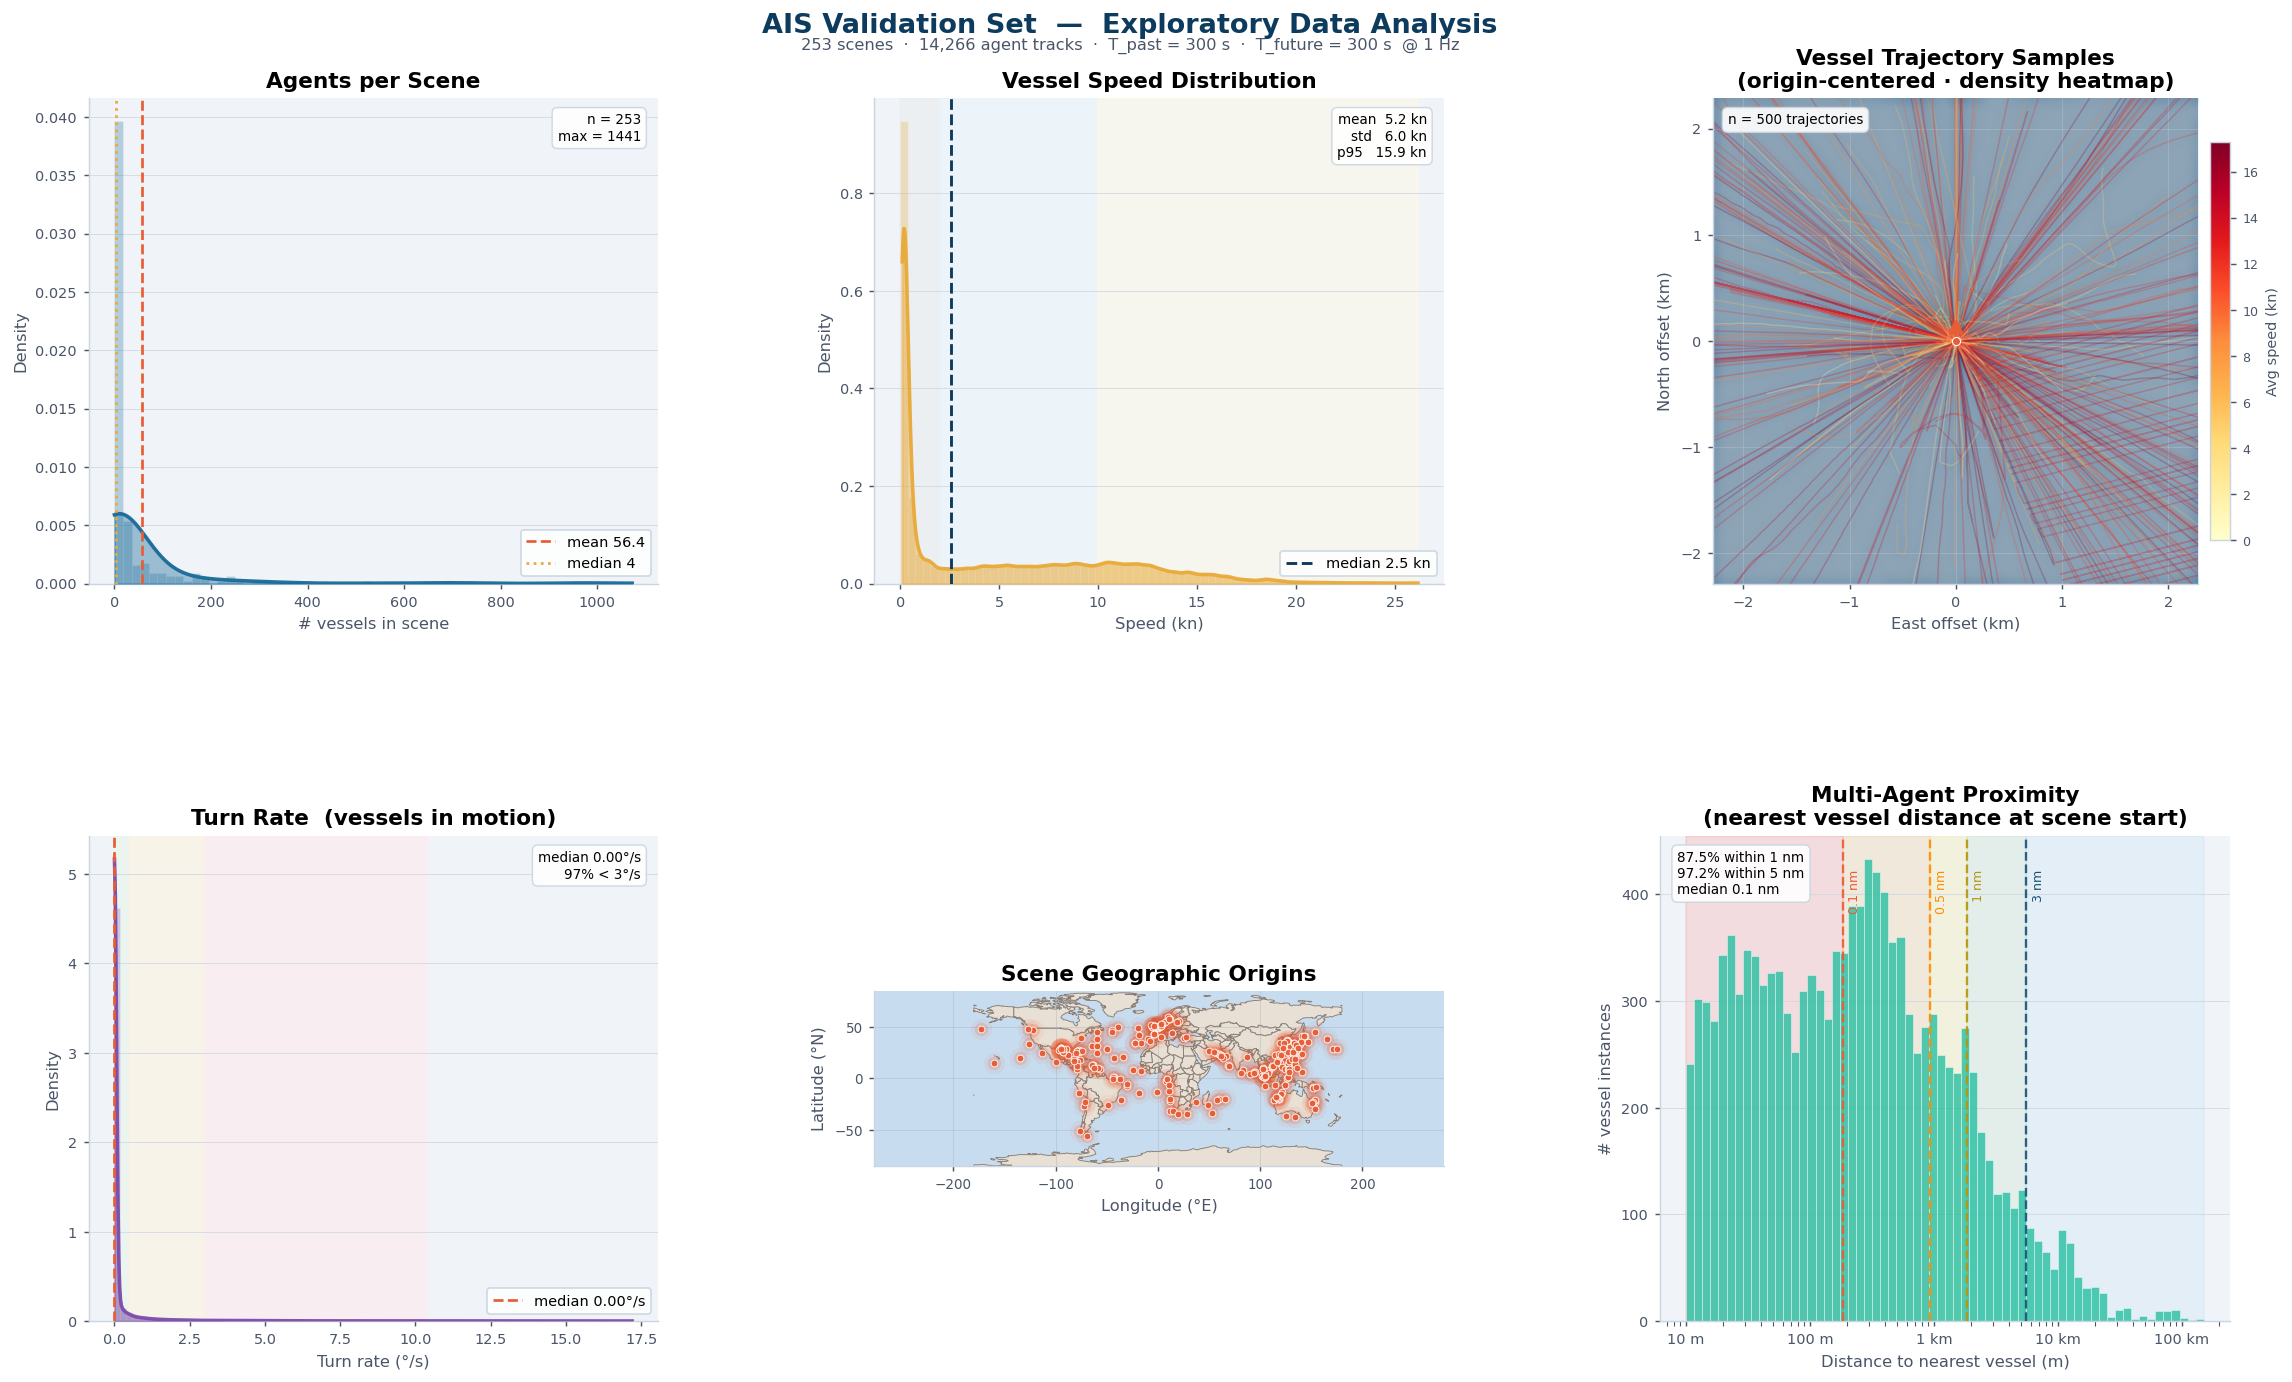
\includegraphics[width=\linewidth]{figures/eda_dashboard.png}
      \caption{Validation-split overview (250 scenes, 13{,}820 vessel instances).
      From left to right: agent count per scene, speed distribution, origin-centred
      trajectory samples coloured by average speed, turn-rate distribution,
      geographic coverage, and nearest-vessel proximity (dashed lines mark
      0.1/0.5/1/3 nm COLREG thresholds).}
      \label{fig:eda_dashboard}
  \end{figure}

  % ─────────────────────────────────────────────────────────────────────────────
\section{Methods}
\label{sec:methods}

This section describes the five approaches compared in this work.
The \textbf{Baseline Linear} model is a parameter-free least-squares
extrapolator that provides a deterministic lower bound on achievable
accuracy.
\textbf{TrAISformer}~\citep{nguyen2021traisformer} is a GPT-style
autoregressive transformer from the maritime literature that predicts
trajectories as sequences of discrete tokens.
\textbf{AIS-ACNet}~\citep{shin2024aisacnet} is a dilated causal CNN
from the maritime literature that processes the past trajectory with
exponentially-dilated convolutions.
\textbf{Wayformer-AIS} is our adaptation of the Wayformer
Perceiver-based architecture~\citep{nayakanti2022wayformer}, originally
developed for road vehicles, which encodes multi-agent social context
via cross-attention.
\textbf{GAT-LSTM}~\citep{zhao2023gatlstm} is a hybrid spatial-temporal
architecture combining a Graph Attention Network (GAT) for spatial
feature extraction with an LSTM for temporal modelling.
All models are trained and evaluated on the same data split with
a fixed random seed of 42 (Section~\ref{sec:training_protocol}).

%─────────────────────────────────────────────────────────────────────────────
\subsection{Baseline Linear (Least-Squares Extrapolation)}
\label{sec:baseline_linear}

The Baseline Linear model serves as the simplest valid lower bound: it
requires no training and makes no assumptions about inter-vessel
interactions.  Given the full sequence of past positions
$\{(x_t, y_t)\}_{t=1}^{T_{\text{past}}}$ for a vessel, the model fits
a linear trend by ordinary least squares (OLS):
\begin{equation}
  \hat{x}(t) = a_x \cdot t + b_x, \quad
  \hat{y}(t) = a_y \cdot t + b_y,
  \label{eq:ols}
\end{equation}
where the slope and intercept are estimated over all valid (unmasked) past
timesteps using mean-centred regression:
\begin{equation}
  a = \frac{\sum_{t \in \mathcal{V}} (t - \bar{t})(p_t - \bar{p})}
           {\sum_{t \in \mathcal{V}} (t - \bar{t})^2}, \quad
  b = \bar{p} - a\,\bar{t},
  \label{eq:ols_coeff}
\end{equation}
where $\mathcal{V}$ is the set of valid timestep indices, $\bar{t}$ is
their mean, and $\bar{p}$ is the mean position.  The extrapolation to
future timestep $t' \in \{T_{\text{past}}+1, \dots,
T_{\text{past}}+T_{\text{future}}\}$ follows directly from
Equation~\eqref{eq:ols}.

The model is implemented as a PyTorch Lightning module with a single
dummy parameter for framework compatibility.  It produces a single
deterministic trajectory ($K=1$); for metric consistency with
$K=6$ models, all six ``modes'' are set to this trajectory and
$\pi_1 = 1, \pi_{2:6} = 0$.  No gradient is propagated through the
prediction.

The Baseline Linear is particularly informative for short horizons, where
vessel motion is approximately linear.  Significant degradation of its
performance in dense or manoeuvring scenarios motivates the need for
interaction-aware learning.

%─────────────────────────────────────────────────────────────────────────────
\subsection{TrAISformer (Autoregressive Transformer)}
\label{sec:traisformer}

TrAISformer~\citep{nguyen2021traisformer} is a GPT-style causal
transformer that treats vessel trajectory prediction as a discrete
sequence-to-sequence problem.  Rather than regressing continuous
coordinates, it quantises each timestep into a \emph{fourhot} token:
four independent categorical distributions over $\Delta x$, $\Delta y$,
SOG, and COG, each discretised into a fixed vocabulary.  The
concatenated logit vector is fed as input to a stack of causally masked
multi-head self-attention blocks, and the model is trained to predict the
next token autoregressively.

\paragraph{Fourhot quantisation.}
We work in the UniTraj ego-relative coordinate frame (positions
normalised by $s_p = 100$\,m, velocities by $s_v = 20$\,m/s).
Empirical p99.9 ranges over the training corpus yield
$x, y \in [-31, 31]$\,hm, so we allocate 256 uniform bins per
spatial axis ($\approx 24$\,m resolution), 30 SOG bins spanning
0--1 normalised speed ($\approx 0.67$\,m/s per bin), and 72 COG bins
spanning $[-\pi, \pi]$ (5$^{\circ}$/bin, matching the original paper).
The per-timestep vocabulary is $256 + 256 + 30 + 72 = 614$ logits.

\paragraph{Architecture.}
The adapted model uses $L=8$ transformer layers, $H=8$ attention heads,
and embedding dimension $d=256$, with dropout $p=0.1$.
A causal mask restricts each position to attend only to previous tokens,
enforcing a temporally consistent autoregressive factorisation.
The context window spans $T_{\text{past}} + T_{\text{future}} = 600$
tokens.

\paragraph{Multi-modal inference.}
To produce $K=6$ modes for comparison with the other models on
minADE$_6$/minFDE$_6$, we perform $K$ independent autoregressive rollouts
with temperature sampling ($\tau = 1.0$).
Modes are treated as equally probable ($\pi_k = 1/K$) since TrAISformer
does not output explicit mode weights.

\paragraph{Training objective.}
The loss is the sum of four per-channel cross-entropy terms, masked to
contribute only from future timesteps:
\begin{equation}
  \mathcal{L}_{\text{TR}} =
  \text{CE}(\hat{q}_x, q_x) + \text{CE}(\hat{q}_y, q_y) +
  \text{CE}(\hat{q}_{\text{sog}}, q_{\text{sog}}) +
  \text{CE}(\hat{q}_{\text{cog}}, q_{\text{cog}}),
  \label{eq:traisformer_loss}
\end{equation}
where $q_{\bullet}$ denotes the target bin index and $\hat{q}_{\bullet}$
the predicted logits.

\paragraph{Adaptation to the 5-minute regime.}
The original model was designed for 10-minute sampling intervals and
3--15\,hour prediction horizons~\citep{nguyen2021traisformer}.
Our regime (1\,Hz, 5-min past and future) produces 600-token sequences,
increasing self-attention cost approximately 31$\times$ per layer.
The model operates as a single-agent (marginal) predictor: only the ego
vessel's past trajectory is provided as context; surrounding vessels are
ignored.

\begin{table}[H]
  \centering
  \caption{TrAISformer hyperparameters.}
  \label{tab:traisformer_hp}
  \begin{tabular}{lc}
    \toprule
    \textbf{Hyperparameter} & \textbf{Value} \\
    \midrule
    Transformer layers $L$         & 8 \\
    Attention heads $H$            & 8 \\
    Embedding dimension $d$        & 256 \\
    Dropout                        & 0.1 \\
    Spatial bins (x, y)            & 256 each \\
    SOG bins                       & 30 \\
    COG bins                       & 72 \\
    Modes $K$ (inference)          & 6 \\
    Sample temperature $\tau$      & 1.0 \\
    Optimizer                      & AdamW \\
    Learning rate                  & $6 \times 10^{-4}$ \\
    LR schedule                    & Cosine annealing \\
    Gradient clip norm             & 1 \\
    Max epochs                     & 100 \\
    Train batch size               & 8 \\
    \bottomrule
  \end{tabular}
\end{table}

%─────────────────────────────────────────────────────────────────────────────
\subsection{Wayformer-AIS}
\label{sec:wayformer}

Wayformer-AIS is our primary model, adapting the Wayformer
architecture~\citep{nayakanti2022wayformer} --- originally developed for
road-vehicle trajectory prediction on the Waymo Open Motion Dataset ---
to the maritime domain. The key architectural insight of Wayformer is
that a Perceiver-based bottleneck encoder-decoder, using factorized
attention over agents and time, achieves state-of-the-art performance
with a simple, scalable design that requires no hand-crafted
scene representations.

\subsubsection{Input Representation and Normalization}
\label{sec:normalization}

Each agent $i$ is represented as a sequence of 39-dimensional feature
vectors over $T_{\text{past}} = 300$ timesteps. The feature vector at
each timestep encodes position, velocity, heading, speed magnitude,
and a binary validity flag. To bring all features into a comparable
numerical range, positions are normalized by a scale of
$s_p = 100$\,m and velocities by $s_v = 20$\,m/s:
\begin{equation}
    \tilde{x} = x / s_p, \quad
    \tilde{y} = y / s_p, \quad
    \tilde{v}_x = v_x / s_v, \quad
    \tilde{v}_y = v_y / s_v.
    \label{eq:normalization}
\end{equation}
Up to $M = 10$ vessels are included per scene. Unlike road-domain
applications of Wayformer, no map or lane information is used; the
map input branch receives a dummy zero tensor and contributes no
meaningful signal to the encoder.

\subsubsection{Encoder}
\label{sec:encoder}

Agent features are first linearly projected into a $d_k = 256$
dimensional embedding space:
\begin{equation}
    \mathbf{e}_i^t = \text{SELU}\!\left(\mathbf{W}_a \mathbf{x}_i^t + \mathbf{b}_a\right)
    + \boldsymbol{\psi}_i^{\text{agent}}
    + \boldsymbol{\psi}_t^{\text{time}},
    \label{eq:agent_emb}
\end{equation}
where $\boldsymbol{\psi}_i^{\text{agent}} \in \mathbb{R}^{d_k}$ and
$\boldsymbol{\psi}_t^{\text{time}} \in \mathbb{R}^{d_k}$ are learnable
positional embeddings for the agent index and time index respectively.
The resulting agent embeddings are flattened across agents and timesteps
to form a sequence $\mathbf{Z} \in \mathbb{R}^{(M \cdot T_{\text{past}}) \times d_k}$.

This sequence is passed to a \textbf{Perceiver Encoder}~\citep{nayakanti2022wayformer}
with $N_{\text{enc}} = 192$ trainable latent queries and
$L_{\text{enc}} = 2$ cross-attention layers. Each cross-attention
layer has $H = 4$ heads with a feedforward hidden size of 1024,
followed by layer normalisation and dropout ($p = 0.1$). The cross-attention
compresses the full $(M \cdot T_{\text{past}})$-length token sequence
into a fixed-size context matrix
$\mathbf{C} \in \mathbb{R}^{N_{\text{enc}} \times d_k}$, regardless
of the number of agents or timesteps present. This bottleneck design
provides robustness to variable scene sizes and missing observations.

\subsubsection{Decoder}
\label{sec:decoder}

The decoder is a \textbf{Perceiver Decoder} with
$N_{\text{dec}} = 128$ trainable output queries and $L_{\text{dec}} = 8$
cross-attention layers. Each output query attends to the context matrix
$\mathbf{C}$ through cross-attention, followed by self-attention among
the output queries themselves, producing an output sequence
$\mathbf{Q} \in \mathbb{R}^{N_{\text{dec}} \times d_k}$.

The first $c = 6$ rows of $\mathbf{Q}$ correspond to the $K = 6$
prediction modes. Two lightweight heads are applied to each mode query:
\begin{align}
    \boldsymbol{\pi} &= \text{softmax}\!\left(\mathbf{W}_p \mathbf{Q}_{1:c}\right)
    \in \mathbb{R}^{c}, \label{eq:mode_prob} \\
    \hat{\mathbf{Y}} &= \mathbf{W}_o \mathbf{Q}_{1:c} \in \mathbb{R}^{c \times T_{\text{future}} \times 5},
    \label{eq:traj_out}
\end{align}
where $\boldsymbol{\pi}$ are mode probabilities and $\hat{\mathbf{Y}}$
contains, for each mode $k$ and future timestep $t$, the parameters of
a bivariate Gaussian: $(\mu_x,\, \mu_y,\, \log\sigma_x,\, \log\sigma_y,\, \rho)$.

\subsubsection{Loss Function}
\label{sec:loss}

Training minimizes a combined regression and classification loss
following the GMM formulation of~\citet{nayakanti2022wayformer}.
For each sample in a batch, the mode $k^*$ geometrically closest
to the ground-truth future trajectory is selected:
\begin{equation}
    k^* = \arg\min_{k} \sum_{t=1}^{T_{\text{future}}}
    m_t \cdot \left\| \hat{\boldsymbol{\mu}}_t^{(k)} - \mathbf{p}_t \right\|_2,
    \label{eq:nearest_mode}
\end{equation}
where $m_t$ is the validity mask. The \textbf{regression loss} is the
negative log-likelihood of the ground truth under the bivariate Gaussian
of mode $k^*$:
\begin{equation}
    \mathcal{L}_{\text{reg}} = \sum_{t=1}^{T_{\text{future}}} m_t \left[
    \log\sigma_x + \log\sigma_y + \tfrac{1}{2}\log(1 - \rho^2)
    + \frac{1}{2(1-\rho^2)} \left(
        \frac{d_x^2}{\sigma_x^2} + \frac{d_y^2}{\sigma_y^2}
        - \frac{2\rho\, d_x d_y}{\sigma_x \sigma_y}
    \right)\right],
    \label{eq:reg_loss}
\end{equation}
where $d_x = \mu_x^{(k^*)} - p_x$ and $d_y = \mu_y^{(k^*)} - p_y$
are the residuals, and $\log\sigma$ values are clipped to
$[-1.609,\, 5.0]$ for numerical stability. The \textbf{classification
loss} trains mode probabilities with cross-entropy:
\begin{equation}
    \mathcal{L}_{\text{cls}} = -\log \pi_{k^*}.
    \label{eq:cls_loss}
\end{equation}
The total loss is:
\begin{equation}
    \mathcal{L} = \frac{1}{B}\sum_{i=1}^{B}
    \left(\mathcal{L}_{\text{reg}}^{(i)} + \mathcal{L}_{\text{cls}}^{(i)}\right).
    \label{eq:total_loss}
\end{equation}

\subsubsection{Maritime Adaptations}
\label{sec:adaptations}

Table~\ref{tab:adaptation} summarises the modifications applied to the
original Wayformer to accommodate the maritime domain.

\begin{table}[H]
    \centering
    \caption{Wayformer adaptations for the maritime domain.}
    \label{tab:adaptation}
    \begin{tabular}{lll}
        \toprule
        \textbf{Aspect} & \textbf{Road (original)} & \textbf{AIS (this work)} \\
        \midrule
        Map input         & Road network / lane polylines & None (dummy zero tensor) \\
        Coordinate frame  & World absolute               & Ego-relative (meters) \\
        Max agents        & 32                           & 10 \\
        Position scale    & Scene-relative               & 100\,m \\
        Velocity scale    & km/h                         & m/s ($\div$\,20) \\
        Agent feature dim & 39                           & 39 (compatible) \\
        \bottomrule
    \end{tabular}
\end{table}

  Figures~\ref{fig:wayformer_manoeuvre} and~\ref{fig:wayformer_anchor} present two
  qualitatively distinct validation scenarios that illustrate the multi-modal output
  of Wayformer-AIS and its ability to capture different maritime motion regimes.

  \paragraph{Scenario~1 --- Active manoeuvre (Figure~\ref{fig:wayformer_manoeuvre}).}
  Vessel~A is observed completing a $+45^{\circ}$ port turn over an
  862\,m past path.  The model produces $K=6$ candidate future trajectories, each
  with a distinct softmax probability $\pi_k$.  The highest-weighted mode (mode~4,
  $p=25\%$, purple) predicts a near-straight continuation consistent with the vessel
  easing out of the turn, while lower-probability modes span alternative headings ---
  port deviations, starboard corrections, and wider arcs.  The ground-truth future
  (green, $+8^{\circ}$ port) falls squarely within the predicted fan, confirming that the
  model correctly frames an ongoing manoeuvre as a \emph{distribution} over plausible
  future headings.  Two consecutive timestamps of the same vessel are shown, both
  exhibiting consistent multi-modal spread across the turn.  This probabilistic
  coverage is the key structural advantage of Wayformer-AIS over the single-mode
  models (AIS-ACNet, GAT-LSTM) and directly enables the Brier-FDE calibration metric.

  \begin{figure}[H]
    \centering
    \begin{subfigure}[b]{0.48\textwidth}
      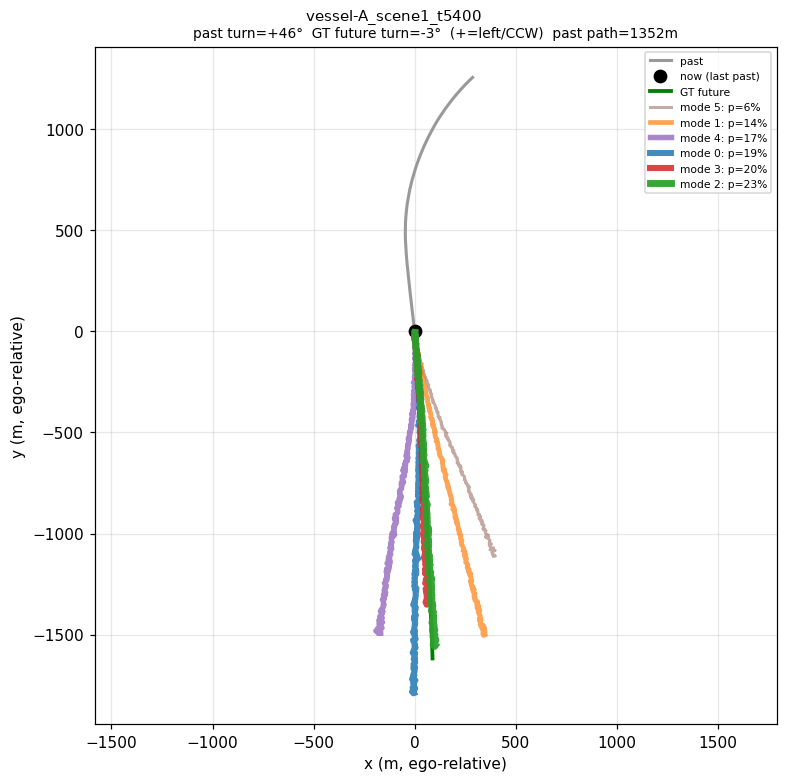
\includegraphics[width=\textwidth]{figures/modes_06_vesselA_t5400}
      \caption{Offset $t=5400$\,s}
    \end{subfigure}
    \hfill
    \begin{subfigure}[b]{0.48\textwidth}
      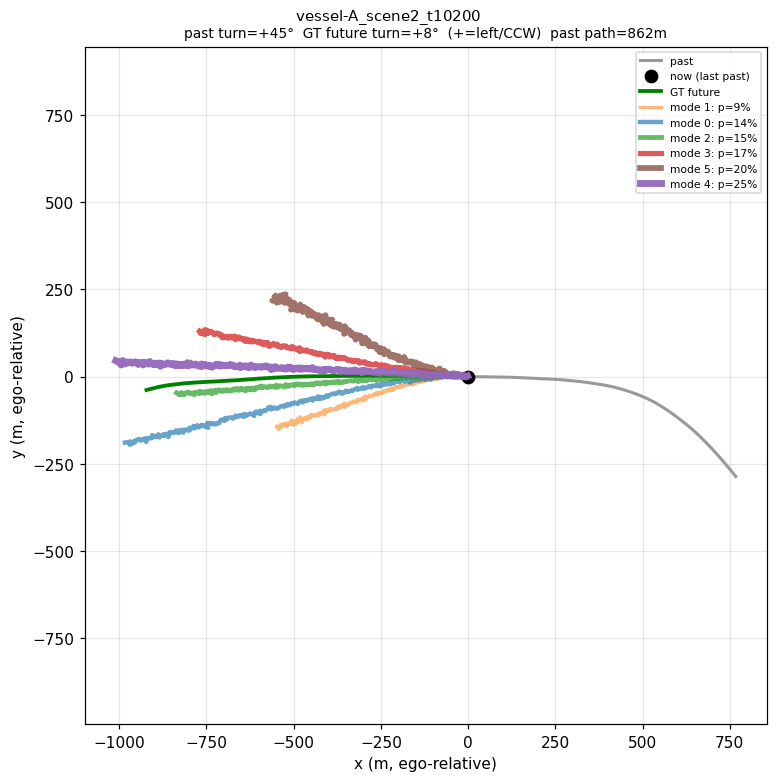
\includegraphics[width=\textwidth]{figures/modes_07_vesselA_t10200}
      \caption{Offset $t=10200$\,s}
    \end{subfigure}
    \caption{Wayformer-AIS predictions for Vessel~A (2024-01-01)
             at two timestamps during an active port-turn manoeuvre
             (past path $=862$\,m, past turn $=+45^{\circ}$ CCW, GT future turn $=+8^{\circ}$).
             \textbf{Gray}: past trajectory.
             \textbf{Black dot}: current position (ego-relative origin).
             \textbf{Green}: ground-truth future.
             \textbf{Coloured}: six predicted modes ($p=9\%$--$25\%$).
             The fan of modes across port and starboard headings reflects
             genuine uncertainty in the vessel's intended manoeuvre.}
    \label{fig:wayformer_manoeuvre}
  \end{figure}

  \paragraph{Scenario~2 --- Deceleration and anchoring (Figure~\ref{fig:wayformer_anchor}).}
  Vessel~B approaches its anchor point after a $-156^{\circ}$ heading
  change over 332\,m of past travel.  The critical signal is in the spacing of
  position fixes in the final seconds of the past window: the AIS points crowd
  tightly together near the current position, a direct kinematic signature of rapid
  deceleration at 1\,Hz resolution.  Wayformer-AIS recognises this pattern and
  responds with a striking prediction: \emph{all six modes cluster within
  approximately 20\,m of the current position}, and the dominant mode (mode~3,
  $p=35\%$) predicts essentially zero future displacement.  The model has inferred,
  purely from velocity and position features in the AIS stream, that the vessel is
  coming to rest.  The ground-truth future (green) confirms this --- the vessel
  anchors and remains nearly stationary for the entire 300\,s forecast horizon.
  Note that the axis range in Figure~\ref{fig:wayformer_anchor} is only $\pm$50\,m,
  an order of magnitude smaller than the manoeuvring scenario above, which visually
  underscores how tightly the model constrains the forecast when it detects a
  stopping vessel.  This example demonstrates that Wayformer-AIS captures not only
  directional uncertainty but also speed dynamics, distinguishing cruising,
  manoeuvring, and anchoring regimes without any explicit navigation-status input.

  \begin{figure}[H]
    \centering
    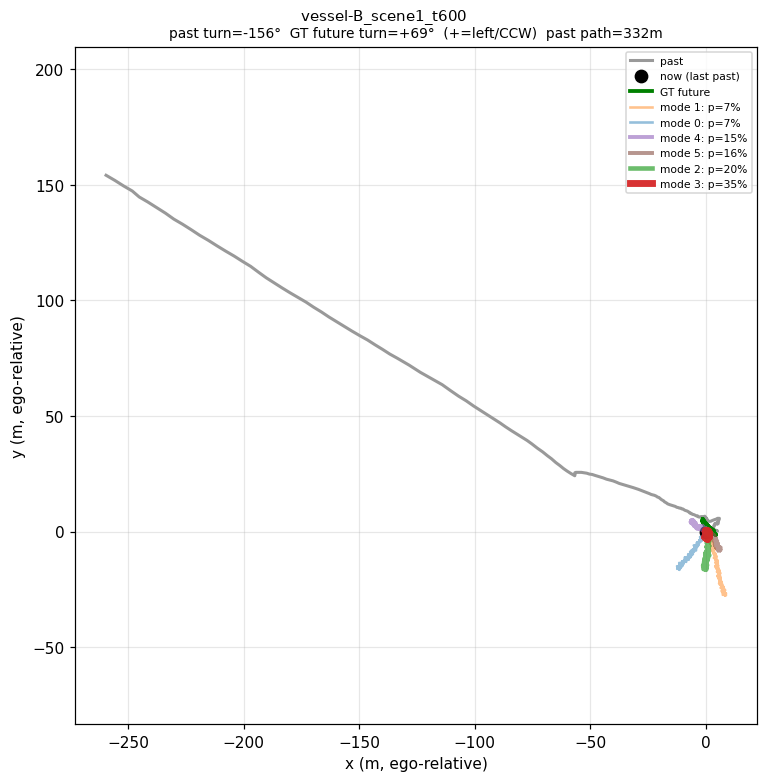
\includegraphics[width=0.60\textwidth]{figures/modes_00_vesselB_t600}
    \caption{Wayformer-AIS prediction for Vessel~B (2024-01-04)
             approaching anchor (past path $=332$\,m, past turn $=-156^{\circ}$).
             \textbf{Gray}: past trajectory --- note the tightly-spaced position
             fixes near the current position, signalling rapid deceleration.
             \textbf{Green}: ground-truth future, confirming near-zero displacement
             over the 300\,s horizon.
             \textbf{Coloured}: all six predicted modes ($p=7\%$--$35\%$)
             cluster within $\approx\!20$\,m of the origin.
             The axis range ($\pm$50\,m) is an order of magnitude smaller than
             Figure~\ref{fig:wayformer_manoeuvre}, highlighting the model's
             ability to predict an imminent anchoring event from kinematic
             features alone.}
    \label{fig:wayformer_anchor}
  \end{figure}

%─────────────────────────────────────────────────────────────────────────────
\subsection{AIS-ACNet (Dilated Causal CNN)}
\label{sec:acnet}

AIS-ACNet~\citep{shin2024aisacnet} predicts vessel trajectories using a
\emph{dual-encoder dilated causal convolutional network} (GWNet backbone).
The architecture processes the past trajectory sequence with two parallel
1-D dilated causal CNN stacks --- one for position ($x$, $y$) and one for
kinematics (SOG, COG) --- whose intermediate activations are fused via
gated residual connections at every layer.

\paragraph{Exponential dilations.}
The network stacks $N=10$ dilated causal convolution layers with
exponential dilation factors $[1, 2, 4, 8, 16, 32, 64, 128, 256, 512]$
and kernel size $k=2$.
The theoretical receptive field is
$1 + (k-1)\sum_{i=1}^{N} d_i = 1 + 1023 = 1024$ timesteps,
fully covering the 300-step past horizon with margin.
The original paper used a smaller dilation schedule designed for its
15-step window; our exponential schedule is the key adaptation for the
5-minute / 1\,Hz regime.

\paragraph{Architecture.}
Each layer has residual channels $C_r = 32$ and dilation channels
$C_d = 32$; skip connections from all layers are summed into a skip
aggregation with $C_s = 256$ channels, followed by a two-layer output
head with $C_e = 512$ intermediate channels.
Total trainable parameters: approximately 1.2\,M.
The model is single-mode (deterministic): it outputs one future
trajectory ($K=1$), so all six ``modes'' are identical when computing
minADE$_6$ and minFDE$_6$.

\paragraph{Training objective.}
Following the original paper, the loss combines MSE on future positions
with two auxiliary SOG and COG regression terms:
\begin{equation}
  \mathcal{L}_{\text{ACN}} = \mathcal{L}_{\text{pos}}
                + \alpha\,\mathcal{L}_{\text{SOG}}
                + \beta\,\mathcal{L}_{\text{COG}},
  \quad \alpha = \beta = 0.2.
  \label{eq:acnet_loss}
\end{equation}

\begin{table}[H]
  \centering
  \caption{AIS-ACNet hyperparameters.}
  \label{tab:acnet_hp}
  \begin{tabular}{lc}
    \toprule
    \textbf{Hyperparameter} & \textbf{Value} \\
    \midrule
    Dilation factors                    & $[1,2,4,8,16,32,64,128,256,512]$ \\
    Residual / dilation channels $C_r$  & 32 \\
    Skip channels $C_s$                 & 256 \\
    Output head channels $C_e$          & 512 \\
    Kernel size                         & 2 \\
    Dropout                             & 0.3 \\
    Modes $K$                           & 1 (deterministic) \\
    Auxiliary loss weights $\alpha,\beta$ & 0.2 \\
    Optimizer                           & Adam \\
    Learning rate                       & $10^{-3}$ \\
    LR decay epochs                     & 80, 90 \\
    Weight decay                        & $10^{-4}$ \\
    Gradient clip norm                  & 5 \\
    Max epochs                          & 100 \\
    Train batch size                    & 32 \\
    \bottomrule
  \end{tabular}
\end{table}


%─────────────────────────────────────────────────────────────────────────────
\subsection{GAT-LSTM (Graph Attention Network + LSTM)}
\label{sec:gatlstm}

GAT-LSTM~\citep{zhao2023gatlstm} combines a Graph Attention Network
(GAT) for spatial feature extraction with a Long Short-Term Memory
(LSTM) network for temporal modelling.  The method was proposed by
\citet{zhao2023gatlstm} for ship trajectory prediction on Chinese
coastal AIS data; we adapt it here to the 5-minute horizon used
throughout this benchmark.

\paragraph{Graph construction.}
The ego vessel's past trajectory is partitioned into contiguous
sub-segments, each forming a node in a directed graph $G = (P, E)$.
Two nodes $i$ and $j$ are adjacent when their sub-segments are
temporally consecutive, yielding an adjacency matrix
$A \in \{0,1\}^{P \times P}$ with a self-loop added to every node:
$\tilde{A} = A + I$.

\paragraph{Spatial encoder (GAT).}
At each timestep the GAT layer computes attention coefficients between
node $i$ and its neighbours $\mathcal{N}(i)$:
\begin{equation}
  \alpha_{ij} =
    \frac{\exp\!\bigl(\text{LeakyReLU}(e_{ij})\bigr)}
         {\sum_{k \in \mathcal{N}(i)} \exp\!\bigl(\text{LeakyReLU}(e_{ik})\bigr)},
  \quad
  e_{ij} = a\!\left(W h_i^l,\; W h_j^l\right),
  \label{eq:gat_attn}
\end{equation}
where $h_i^l \in \mathbb{R}^F$ is the node-$i$ feature at GAT layer $l$,
$W \in \mathbb{R}^{F' \times F}$ is a learnable weight matrix, and
$a(\cdot)$ is a shared attention function.  Updated node features are:
\begin{equation}
  h_i^{l+1} = \sigma\!\left(\sum_{j \in \mathcal{N}(i)} \alpha_{ij}\, W h_j^l\right).
  \label{eq:gat_update}
\end{equation}
Multi-head attention with $K_{\text{heads}} = 4$ independent mechanisms
is applied; their outputs are concatenated before being passed to the
LSTM.

\paragraph{Temporal decoder (LSTM).}
The GAT-encoded feature at each past timestep is fed sequentially into
a 2-layer LSTM with hidden size 128.  The final hidden state
$h_{T_{\text{past}}}$ is projected by a linear layer to a flat vector,
then reshaped to $T_{\text{future}} \times 2$ predicted $(x, y)$
positions.  The model is deterministic ($K = 1$); for metric consistency,
all six modes are set to this single trajectory with $\pi_1 = 1$.

\paragraph{Adaptation to the 5-minute regime.}
The original architecture was designed for short prediction horizons
(10\,s -- 1\,min) with next-step autoregressive decoding.
Our adaptation replaces the autoregressive decoder with a direct
multi-step linear projection from the LSTM final hidden state,
predicting all $T_{\text{future}} = 300$ future positions at once.

\begin{table}[H]
  \centering
  \caption{GAT-LSTM hyperparameters.}
  \label{tab:gatlstm_hp}
  \begin{tabular}{lc}
    \toprule
    \textbf{Hyperparameter} & \textbf{Value} \\
    \midrule
    GAT hidden size                        & 32 \\
    GAT layers                             & 2 \\
    Attention heads $K_{\text{heads}}$     & 4 \\
    LSTM hidden size                       & 128 \\
    LSTM layers                            & 2 \\
    Input features                         & 4 ($x,\,y,\,v_x,\,v_y$) \\
    Dropout                                & 0.3 \\
    Modes $K$                              & 1 (deterministic) \\
    Optimizer                              & Adam \\
    Learning rate                          & $10^{-3}$ \\
    LR decay epochs                        & 80, 90 \\
    Weight decay                           & $10^{-4}$ \\
    Gradient clip norm                     & 5 \\
    Max epochs                             & 100 \\
    Train batch size                       & 32 \\
    \bottomrule
  \end{tabular}
\end{table}
%─────────────────────────────────────────────────────────────────────────────
\subsection{Shared Training Protocol}
\label{sec:training_protocol}

All learned models are trained under the following shared conditions to
ensure that performance differences reflect architectural choices rather
than experimental setup.

\paragraph{Data.}
All models are trained and evaluated on the same fixed data split, constructed
according to the procedure described in Section~\ref{sec:pipeline}: each 4-hour
scene is assigned whole to a single split, so that no observation window is
shared between partitions.
A fixed random seed of 42 is used throughout, and the preprocessing pipeline and
normalisation constants ($s_p = 100$\,m, $s_v = 20$\,m/s) are identical across
models.

\paragraph{Uniform evaluation protocol.}
The results in Section~\ref{sec:experiments} are produced by re-evaluating every
model under a single common protocol, rather than by collating the metrics each
model happened to log during its own training run.  All five models are scored
on the complete split with no per-run cap on the number of scenes loaded, using
the same observation and prediction horizons
($T_{\text{past}} = T_{\text{future}} = 300$\,s at 1\,Hz), the same 300\,s
sliding-window stride, the same number of output modes ($K = 6$), and the same
metric implementations.  This yields 11{,}891 prediction windows on the test
split and 10{,}336 on the validation split, and within a split every model is
scored on exactly the same windows.

Enforcing this uniformity is essential to the comparison.  Metrics recorded
during separate training runs are not directly comparable, because those runs
may differ in how many scenes were loaded and in the stride used to extract
windows; a difference between two such figures reflects the evaluation sample as
much as the architecture.  Model selection and reporting are also kept apart:
each checkpoint is chosen on the validation split (see below), while the primary
results are reported on the held-out test split.

\paragraph{Checkpoint selection.}
The best model checkpoint is selected by minimising the validation
Brier-FDE over all training epochs, where
Brier-FDE~\citep{feng2024unitraj} is defined as:
\begin{equation}
  \text{Brier-FDE} = \text{minFDE}_K + (1 - \pi_{k^*})^2,
  \label{eq:brier_fde}
\end{equation}
and $\pi_{k^*}$ is the predicted probability of the best mode.
This metric jointly rewards spatial accuracy and calibrated confidence.

\paragraph{Hardware.}
All learned models are trained on an AWS EC2 \texttt{g5.8xlarge}
instance equipped with a single NVIDIA A10G GPU (24\,GB VRAM),
an AMD EPYC 7R32 CPU (32 vCPUs), and 128\,GB of system RAM.
The Baseline Linear requires no GPU and is evaluated on CPU.

\paragraph{Experiment tracking.}
All training runs and evaluation results across every architecture are logged to a shared project on the Weights~\&~Biases (W\&B)
platform~\citep{wandb2020}.  Each run records per-epoch training and validation
losses, the four evaluation metrics, gradient norms, and hardware utilisation,
providing a single point of visibility for cross-model comparison.  This
centralised tracking was instrumental in identifying the best checkpoint for each
model and in reproducing any reported result from its exact hyperparameter
configuration.

\paragraph{Per-model training details.}
Each model uses its own optimizer and schedule, reflecting best practices
from its source paper.  Table~\ref{tab:training_summary} summarises the
key differences.

\begin{table}[H]
  \centering
  \caption{Per-model training configuration. All models use the same
  data split, seed (42), and checkpoint selection criterion (val/brier\_fde).}
  \label{tab:training_summary}
  \begin{tabular}{lcccc}
    \toprule
    \textbf{Model} & \textbf{Optimizer} & \textbf{LR / Schedule}
                   & \textbf{Epochs} & \textbf{Best ckpt epoch} \\
    \midrule
    Baseline Linear & --- & --- & --- & --- \\
    TrAISformer     & AdamW & $6\!\times\!10^{-4}$ / cosine & 100 & 32 \\
    AIS-ACNet       & Adam  & $10^{-3}$ / step at [80,90]   & 100 & 99 \\
    Wayformer-AIS   & AdamW & $10^{-3}$ / OneCycleLR        & 100 & 96 \\
    GAT-LSTM        & Adam  & $10^{-3}$ / step at [80,90]   & 100 & 20 \\
    \bottomrule
  \end{tabular}
\end{table}

% ─────────────────────────────────────────────────────────────────────────────
  \section{Experiments}
  \label{sec:experiments}

  \subsection{Quantitative Comparison}

  \begin{table}[H]
  \centering
  \small
  \caption{Main results under an identical evaluation protocol for every model
           ($T_{\text{past}} = T_{\text{future}} = 300$\,s, $K=6$, window stride
           300\,s, all scenes in the split, seed 42).
           Upper panel: held-out test set.  Lower panel: validation set.
           $\downarrow$ = lower is better; best learned model in \textbf{bold}.
           The parameter-free OLS baseline is the reference line --- learned models
           that fall below it do not beat constant-velocity extrapolation.}
  \label{tab:main_results}
\resizebox{\textwidth}{!}{%
  \begin{tabular}{lcccccc}
      \toprule
      \textbf{Model}
          & \textbf{minADE$_6$} $\downarrow$
          & \textbf{minFDE$_6$} $\downarrow$
          & \textbf{Brier-FDE} $\downarrow$
          & \textbf{Miss@2\,m} $\downarrow$
          & \textbf{Miss@10\,m} $\downarrow$
          & \textbf{Miss@20\,m} $\downarrow$ \\
          & (m) & (m) & & (\%) & (\%) & (\%) \\
      \midrule
      \multicolumn{7}{l}{\textit{Test set --- 11{,}891 prediction windows}} \\
      Baseline Linear (OLS)  & 26.70 & 51.43 & 51.43 & 95.3 & 68.1 & 45.8 \\
      Wayformer-AIS          & \textbf{15.57} & \textbf{31.71} & \textbf{32.31}
                             & \textbf{91.6} & \textbf{67.3} & \textbf{41.6} \\
      AIS-ACNet$^{\dagger}$  & 27.03 & 56.76 & 56.76 & 96.4 & 78.8 & 65.7 \\
      TrAISformer            & 100.43 & 186.49 & 187.19 & 99.8 & 81.9 & 73.5 \\
      GAT-LSTM$^{\dagger}$   & 409.42 & 819.12 & 819.12 & 100.0 & 100.0 & 99.7 \\
      \midrule
      \multicolumn{7}{l}{\textit{Validation set --- 10{,}336 prediction windows}} \\
      Baseline Linear (OLS)  & 34.19 & 65.85 & 65.85 & 95.7 & 71.3 & 49.9 \\
      Wayformer-AIS          & \textbf{18.07} & \textbf{36.94} & \textbf{37.56}
                             & \textbf{92.7} & \textbf{71.3} & \textbf{44.2} \\
      AIS-ACNet$^{\dagger}$  & 33.13 & 69.90 & 69.90 & 96.2 & 81.1 & 67.6 \\
      TrAISformer            & 101.19 & 188.97 & 189.66 & 99.6 & 85.0 & 77.6 \\
      GAT-LSTM$^{\dagger}$   & 379.23 & 756.05 & 756.05 & 100.0 & 100.0 & 99.5 \\
      \bottomrule
  \end{tabular}}

  \vspace{2pt}
  {\footnotesize $^{\dagger}$ Single-mode by architecture: minADE$_6$ is
  effectively minADE$_1$ and Brier-FDE collapses onto minFDE$_6$.}
\end{table}

  \begin{figure}[H]
    \centering
    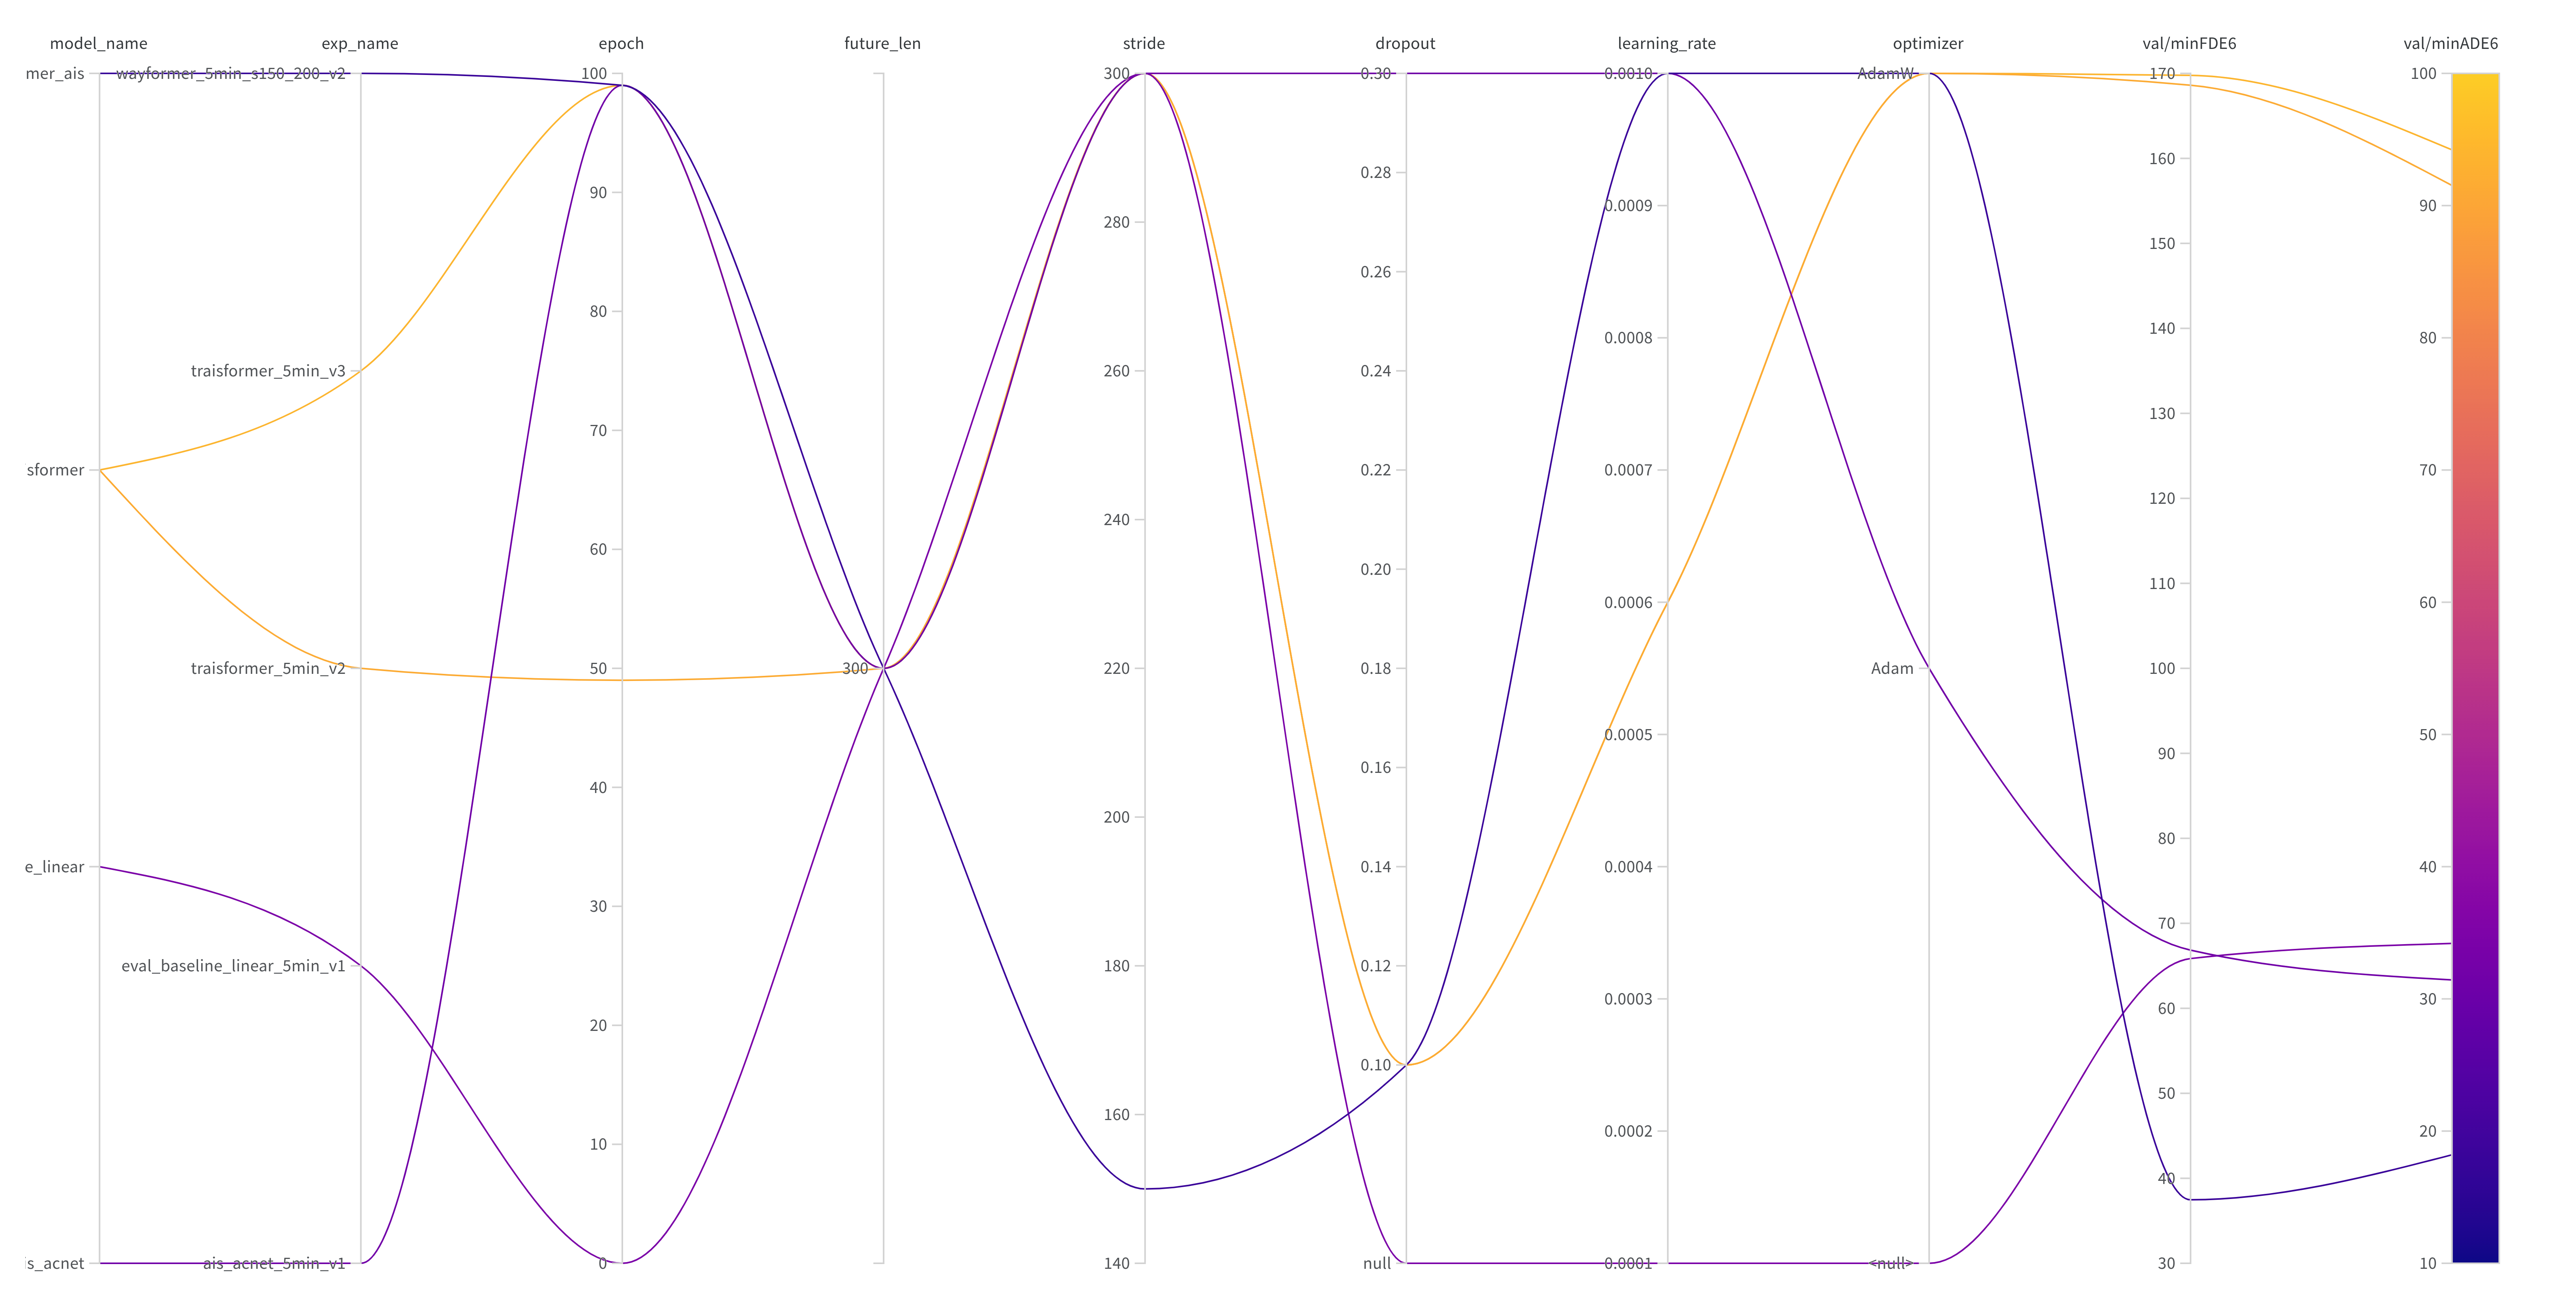
\includegraphics[width=\textwidth]{figures/wandb_parallel_coords}
    \caption{Parallel coordinates view of all model runs on the W\&B experiment
             tracking platform~\citep{wandb2020}.  Each line represents one run;
             axes show key hyperparameters (epoch, future horizon, stride, dropout,
             learning rate, optimiser) and final validation metrics
             (\textit{val/minFDE$_6$}, \textit{val/minADE$_6$}).
             Lines are colour-coded by \textit{val/minADE$_6$}
             (dark~purple~$\rightarrow$~low/good,
              orange~$\rightarrow$~high/poor).
             Wayformer-AIS (bottom-right cluster, dark purple) achieves the lowest
             minADE$_6$ across all runs; GAT-LSTM and TrAISformer runs trail
             significantly in both metrics.}
    \label{fig:wandb_parallel}
  \end{figure}

  \subsection{Performance by Prediction Horizon}
  \label{sec:horizon}

  A single aggregate metric such as minADE$_6$ collapses all 300 future
  timesteps into one number and can obscure where in the prediction window
  each model breaks down.  Figure~\ref{fig:ade_horizon} decomposes that number:
  the prediction horizon is truncated at each of the 300 timesteps in turn and
  minADE$_6$ recomputed there, for all five models on the held-out test split.
  Every point on every curve is therefore measured rather than extrapolated, and
  the value each curve takes at 300\,s reproduces that model's row in
  Table~\ref{tab:main_results}.  The axis stops at five minutes because the evaluation window itself is
  300\,s long: beyond it there is no ground truth to measure against, and every
  learned output head in the comparison is exactly 300 timesteps wide.  A logarithmic ordinate is necessary to accommodate GAT-LSTM's
  error of several hundred metres alongside the other models.

  Several trends emerge from the figure.  First, \textbf{Wayformer-AIS} holds the
  lowest error at effectively every point in the window, from 3.67\,m at one
  minute to 15.57\,m at five, against 9.77\,m and 26.70\,m for the Baseline
  Linear model --- a 1.71$\times$ improvement at the evaluation horizon and a wider
  one earlier.  Second, \textbf{TrAISformer} is worse than constant-velocity
  extrapolation at every timestep without exception, and falls further behind as
  the horizon lengthens: its autoregressive generation accumulates error at each
  decoding step, reaching 100.43\,m at five minutes, nearly four times the
  Baseline.  This behaviour is consistent with the known compounding-error
  pathology of autoregressive sequence models applied to regression
  tasks~\citep{nguyen2021traisformer}.

  Third, \textbf{AIS-ACNet} shows that the ranking at five minutes is not the
  ranking throughout.  It is more accurate than the Baseline Linear model for the
  first 281\,seconds of the window --- 5.84\,m against 9.77\,m at one minute, a
  40\,\% reduction --- and surrenders that advantage only in the final
  19\,seconds, finishing marginally behind on minADE$_6$ (27.03\,m against
  26.70\,m) and more clearly behind on minFDE$_6$ (56.76\,m against 51.43\,m),
  the metric that scores the endpoint alone.  Its error grows faster than the
  kinematic reference even while it remains below it, so the dilated causal
  convolution buys a real but temporary advantage, one that has expired by the
  horizon at which the comparison is scored.  This is the decomposition earning
  its place: an aggregate at 300\,s records AIS-ACNet as a model that does not
  beat constant velocity, while the curve shows it beating constant velocity for
  94\,\% of the window and losing on the approach to the endpoint.  Against
  that, Wayformer-AIS is the only model whose margin over the baseline is
  sustained from the first timestep to the last.

  Finally, \textbf{GAT-LSTM} diverges from the outset, reaching 409.42\,m
  minADE$_6$ by five minutes --- a Miss Rate of 100\,\% at the 2\,m and 10\,m
  thresholds confirms the model fails to produce any usable prediction on this
  dataset, likely because its single-step ADE training objective does not
  generalise to 300-step rollouts at 1\,Hz maritime resolution.

  Read against the OLS reference line, these results carry a sharper message than
  a simple ranking.  Of the four learned architectures, \emph{only} Wayformer-AIS
  beats constant-velocity extrapolation at the five-minute evaluation horizon;
  AIS-ACNet, TrAISformer and GAT-LSTM all fall short of it there, on both splits.  That a dilated convolution, an autoregressive
  transformer and a graph-recurrent hybrid each lose to a parameter-free linear
  fit is the most consequential outcome of this comparison: at a five-minute
  maritime horizon, learned sequence modelling does not by itself improve on
  constant-velocity extrapolation, and a study reporting only learned models
  against one another would have concealed that.

  The architectures also differ in what they are permitted to observe, and on
  this axis the field divides cleanly.  AIS-ACNet, TrAISformer and GAT-LSTM are
  all \emph{single-vessel} predictors: each forecasts a ship from its own past
  track, and the presence, bearing and motion of every other vessel in the scene
  are invisible to them.  Wayformer-AIS alone is given the surrounding traffic as
  input, attending over as many as ten vessels in the encounter and forming its
  prediction in the context of the scene rather than of one isolated track.  It
  is, in other words, the only model in this comparison equipped to treat a
  manoeuvre as a response to anything.

  It is also the only one that beats constant-velocity extrapolation at the
  evaluation horizon, and the only one that does so at every point before it.
  The two facts sit together and are, at minimum, mutually consistent: the architecture
  with access to scene context is the architecture that clears the kinematic
  reference line, and it does so by the widest margin in exactly the regimes
  where a vessel's motion is most plausibly shaped by the vessels around it
  (Section~\ref{sec:manoeuvre}).  We state the association rather than a
  mechanism, since interaction-awareness and the winning architecture coincide in
  a single model and the margin in Table~\ref{tab:main_results} reflects that
  architecture as a whole.  What the comparison does establish is narrower but
  not weak: among the designs examined here, the one built to perceive its
  surroundings is the only one whose predictions are worth preferring to a
  straight line.

  \begin{figure}[H]
    \centering
    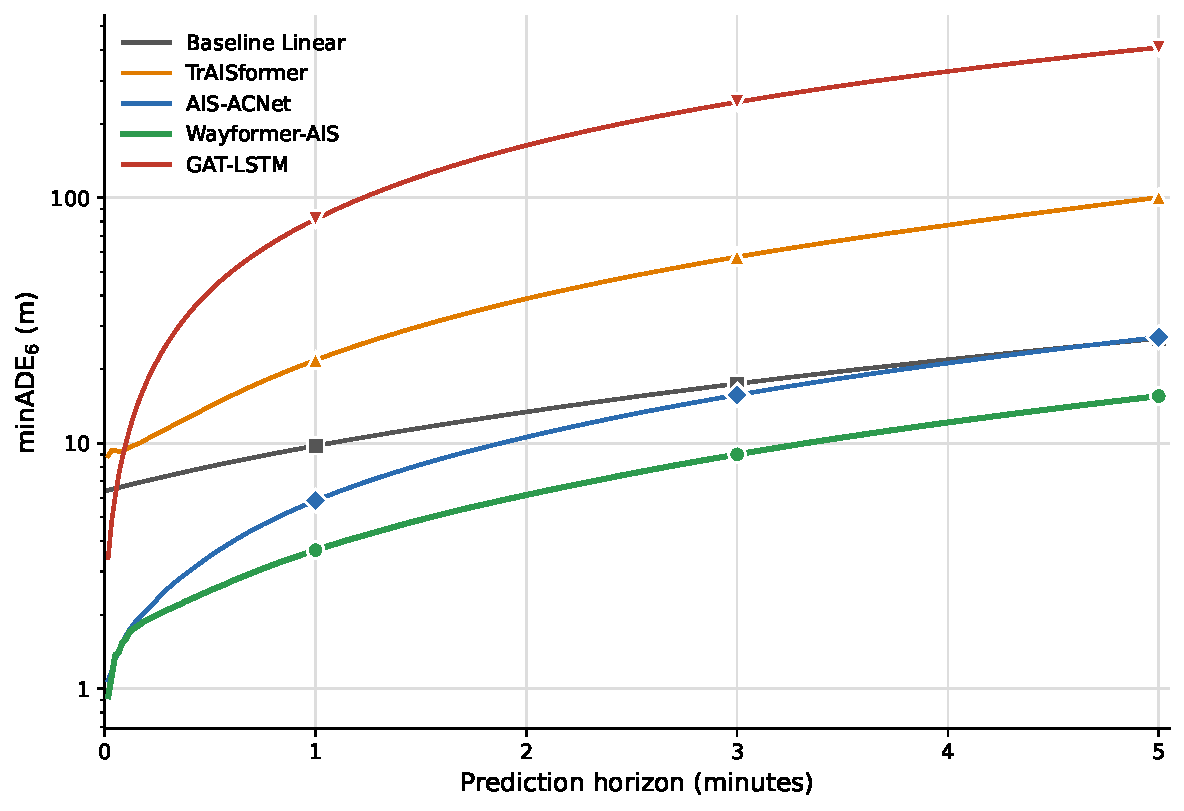
\includegraphics[width=\textwidth]{figures/ade_vs_horizon}
    \caption{minADE$_6$ against prediction horizon for all five models on the
             held-out test split (log scale).  The horizon is truncated at each
             of the 300 timesteps in the window and the metric recomputed there,
             so every point is measured rather than extrapolated; markers
             highlight 1, 3 and 5\,minutes, and the value at 5\,minutes
             reproduces each model's row in Table~\ref{tab:main_results}.
             Wayformer-AIS holds the lowest error across the window; AIS-ACNet
             runs below the Baseline Linear model for the first 281\,s before
             crossing above it; GAT-LSTM diverges from the outset
             ($\text{minADE}_6 = 409.42$\,m at 5\,min, Miss@2\,m\,=\,100\,\%).}
    \label{fig:ade_horizon}
  \end{figure}

  \subsection{Performance by Manoeuvre Regime}
  \label{sec:manoeuvre}

  Aggregate metrics average over every kind of vessel behaviour, from a ship at
  anchor to one executing a hard course alteration.  Because these regimes differ
  by more than an order of magnitude in intrinsic difficulty, an aggregate figure
  can conceal both where a model earns its advantage and where it fails.  We
  therefore stratify the test set by the \emph{ground-truth manoeuvre} performed
  during the prediction window, classifying each window by the total heading
  change of the observed future trajectory: \textbf{stationary} (displacement
  below the AIS noise floor), \textbf{straight} ($<10^{\circ}$),
  \textbf{mild turn} ($10^{\circ}$--$30^{\circ}$) and \textbf{sharp turn}
  ($\geq 30^{\circ}$).  Table~\ref{tab:manoeuvre} reports minFDE$_6$ within each
  regime for all five models, together with each model's margin against the OLS
  baseline evaluated on the identical windows.

  \begin{table}[H]
    \centering
    \small
    \caption{Test-set minFDE$_6$ (m) by ground-truth manoeuvre regime, with each
             model's margin against the OLS baseline on the same windows
             ($\Delta$; negative = better than constant-velocity extrapolation).
             Bucket shares are of the 11{,}891 test windows.}
    \label{tab:manoeuvre}
\resizebox{\textwidth}{!}{%
    \begin{tabular}{lrrrrrrrrr}
      \toprule
      & & \multicolumn{2}{c}{\textbf{Wayformer-AIS}}
        & \multicolumn{2}{c}{\textbf{AIS-ACNet}}
        & \multicolumn{2}{c}{\textbf{TrAISformer}}
        & \multicolumn{2}{c}{\textbf{GAT-LSTM}} \\
      \cmidrule(lr){3-4}\cmidrule(lr){5-6}\cmidrule(lr){7-8}\cmidrule(lr){9-10}
      \textbf{Regime} & \textbf{OLS}
        & minFDE & $\Delta$ & minFDE & $\Delta$
        & minFDE & $\Delta$ & minFDE & $\Delta$ \\
      \midrule
      Stationary (18.5\,\%) & 6.05
        & \textbf{2.84} & $-3.20$ & 6.18 & $+0.13$
        & 8.12 & $+2.08$ & 648.57 & $+642.52$ \\
      Straight (13.6\,\%) & 35.26
        & \textbf{22.25} & $-13.00$ & 48.52 & $+13.26$
        & 181.13 & $+145.88$ & 859.06 & $+823.80$ \\
      Mild turn (60.9\,\%) & 61.31
        & \textbf{38.44} & $-22.87$ & 70.37 & $+9.07$
        & 237.20 & $+175.89$ & 866.01 & $+804.71$ \\
      Sharp turn (6.9\,\%) & 117.71
        & \textbf{68.25} & $-49.46$ & 88.53 & $-29.18$
        & 228.27 & $+110.56$ & 784.59 & $+666.88$ \\
      \bottomrule
    \end{tabular}}
  \end{table}

  \paragraph{The advantage concentrates where extrapolation fails.}
  Wayformer-AIS is the only model that improves on the OLS baseline in
  \emph{every} regime, and the size of that improvement grows monotonically with
  manoeuvre difficulty: $-3.20$\,m on stationary vessels, $-13.00$\,m on straight
  passages, $-22.87$\,m on mild turns and $-49.46$\,m on sharp turns.  The
  advantage is therefore not distributed evenly across the split but concentrates
  in the windows where constant-velocity extrapolation is weakest.  A model that
  merely reproduced the vessel's recent velocity would track the baseline
  everywhere and show a flat margin; the observed gradient shows instead that
  Wayformer-AIS retains useful accuracy precisely where the kinematic assumption
  fails, which is the regime that matters operationally, since it is the
  manoeuvring vessel rather than the steady one that drives a collision-avoidance
  decision.

  \paragraph{The competing architectures fail in diagnostically different ways.}
  AIS-ACNet is \emph{worse} than constant velocity on the easy regimes
  ($+13.26$\,m on straight passages, $+9.07$\,m on mild turns) while beating it on
  sharp turns ($-29.18$\,m): its dilated convolutions capture some curvature but
  at the cost of injecting spurious motion into windows that a straight-line
  extrapolation would have handled correctly.  TrAISformer loses to the baseline
  in every regime, by margins ($+110$ to $+176$\,m) far exceeding the errors being
  measured, consistent with the compounding-error behaviour identified in
  Section~\ref{sec:horizon}.  GAT-LSTM's stationary-regime minFDE$_6$ of
  648.57\,m is the most informative single number in the table: a model that
  forecasts more than half a kilometre of displacement for a vessel that does not
  move has not learned the task in any usable sense, and its apparently
  ``better'' relative performance on sharp turns reflects only that the reference
  errors are larger there.

  \paragraph{A caveat on the bucket boundaries.}
  The mild-turn regime accounts for 60.9\,\% of test windows, which is large for a
  category defined by a $10^{\circ}$ threshold.  Part of this mass reflects
  genuine low-rate course adjustment, and part reflects heading jitter in the AIS
  signal at 1\,Hz resolution; the stationary bucket is separated first precisely
  because reported heading is unreliable at very low speed.  The stratification
  should therefore be read as a difficulty ordering rather than as a
  navigationally exact taxonomy.

  \subsection{Qualitative Analysis}
  \label{sec:qualitative}

  We examine two representative scenarios from the validation set to illustrate
  the behaviour that the aggregate metrics capture only partially.

  \paragraph{Scene 1 --- Dense traffic in the Yellow Sea.}
  Figure~\ref{fig:qual_scene1} shows a ten-vessel scene recorded off the west
  coast of South Korea on 23 September 2024.  Vessel~0 (the prediction target) is
  a large cargo vessel navigating through a congested shipping lane.
  The model produces six hypothesis trajectories; the best mode closely follows the
  ground-truth course alteration, yielding a per-scene \(\ \text{minADE}_6 =
  14.57\,\text{m}\), below the dataset mean of 18.1\,m.  A kinematic baseline
  that projects the most recent heading forward would miss the turn entirely.
  This demonstrates that the cross-vessel attention in Wayformer-AIS extracts
  actionable social context: the presence and relative bearing of nine surrounding
  vessels provides a latent signal that a course change is imminent, consistent
  with COLREG Rule~16 (give-way vessel obligation).

  \begin{figure}[htbp]
    \centering
    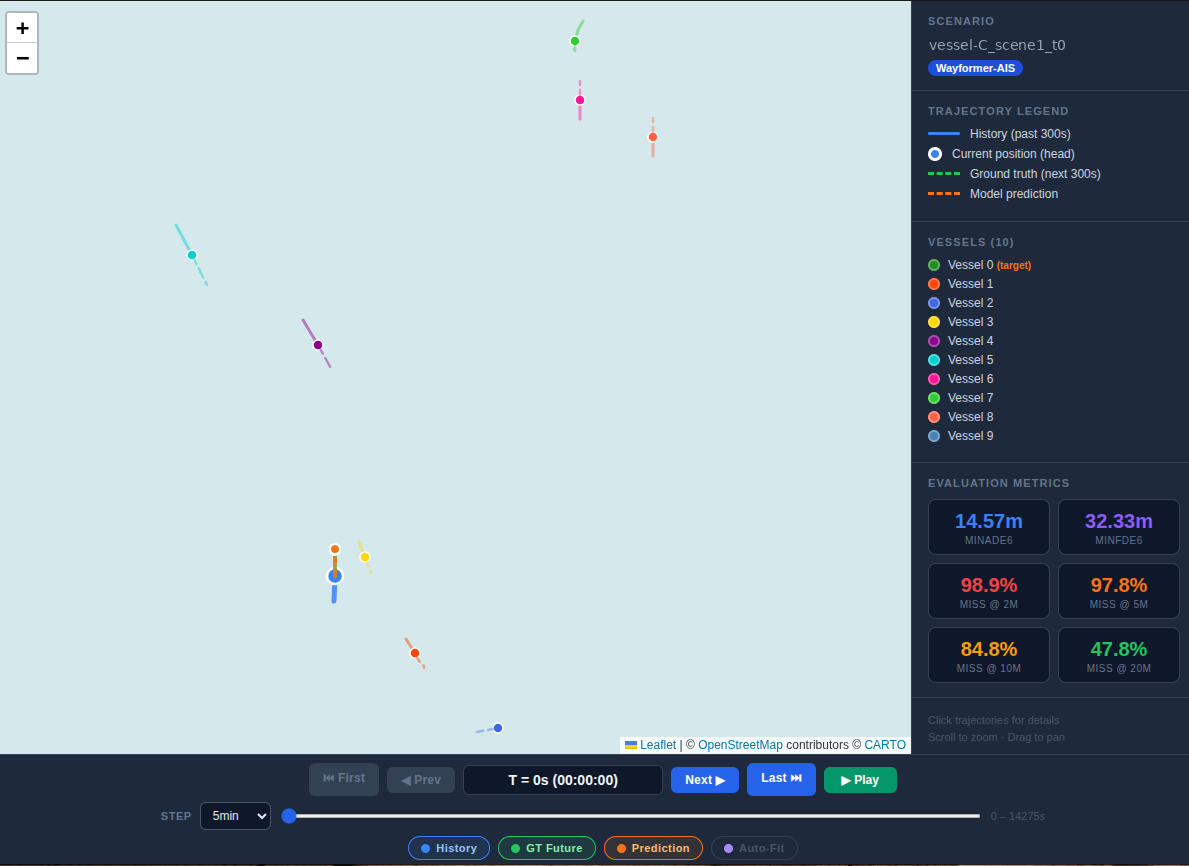
\includegraphics[width=\linewidth]{figures/qual_wayformer_vesselC_scene1.png}
    \caption{Dense ten-vessel scene in the Yellow Sea (23 Sep 2024, scene
    \texttt{vessel-C\_scene1}).
    Solid lines show the 300\,s observation history; green dashed line is the
    ground-truth future; orange dashed lines are the six Wayformer-AIS mode
    predictions.  The best mode captures the vessel's course alteration in a
    congested COLREG environment.
    minADE$_6$ = 14.57\,m, minFDE$_6$ = 32.33\,m.}
    \label{fig:qual_scene1}
  \end{figure}

  \paragraph{Scene 2 --- Stationary vessel during pilot transfer.}
  Figure~\ref{fig:qual_scene2} shows a qualitatively distinct scenario from
  18 November 2024.  Vessel~0 is stationary --- likely waiting at the pilot
  boarding ground outside a port while a second vessel approaches and comes
  alongside to transfer the harbour pilot.  Despite the strong social signal
  from an approaching vessel that would, in most contexts, trigger an evasive
  prediction, Wayformer-AIS correctly predicts near-zero displacement for the
  target.  This is notable: the model has implicitly learned from training data
  that a stationary vessel in close proximity to a small approaching boat does
  not manoeuvre --- a maritime convention with no analogue in road-traffic
  datasets.  The scenario represents an out-of-distribution event that the
  model handles without incident: the observed kinematics of both vessels ---
  one stationary, one closing slowly --- are consistent with a controlled
  approach rather than a developing encounter.

  \begin{figure}[htbp]
    \centering
    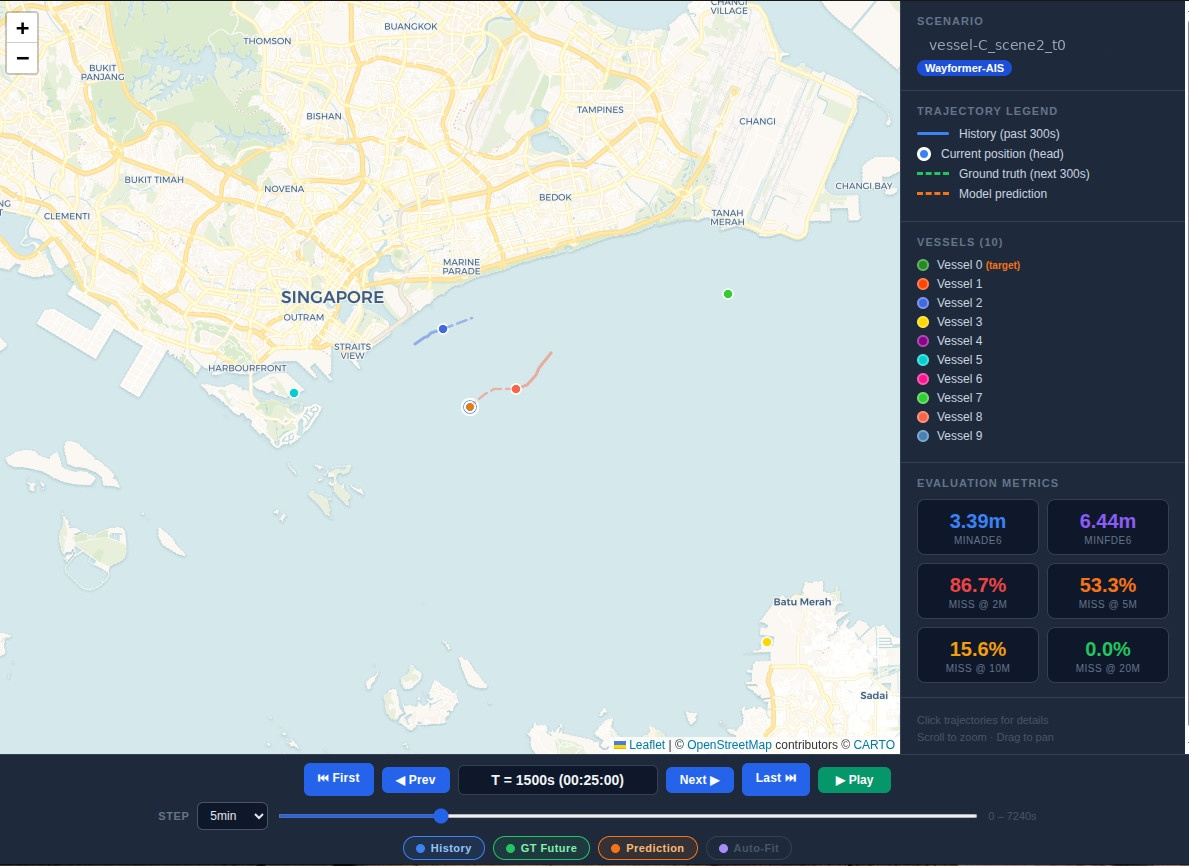
\includegraphics[width=\linewidth]{figures/qual_wayformer_vesselC_scene2.jpg}
    \caption{Singapore Strait scenario (18 Nov 2024, scene
    \texttt{vessel-C\_scene2}).
    Vessel~0 (target, green) is nearly stationary in the strait south of
    Singapore while Vessel~1 (orange) approaches from the east.
    Wayformer-AIS predicts near-zero displacement, consistent with the
    vessel awaiting a pilot or holding position before port entry.
    All six prediction modes remain close to the observed position
    (minADE$_6$ = 3.39\,m, minFDE$_6$ = 6.44\,m).}
    \label{fig:qual_scene2}
  \end{figure}

  \paragraph{Failure modes.}
  Both scenes above are success cases, selected to show what the model does when
  it works.  They are not representative: the miss rate of 91.6\,\% at the
  2\,m threshold on the test set makes clear that most windows are not predicted
  to that tolerance.  Section~\ref{sec:failure} characterises the failures
  systematically rather than anecdotally.

  \subsection{Failure Modes}
  \label{sec:failure}

  An aggregate error figure reports how far a prediction lands from the truth,
  but not what kind of mistake produced that distance.  This section
  characterises the failures of Wayformer-AIS on the held-out test split.

  \paragraph{A turn already in progress is predicted as a straight line.}
  Restricting attention to \emph{moving} windows whose observed past curves by at
  least $15^{\circ}$ --- 156 of the 11{,}891 test windows, or 1.3\,\% --- the ground
  truth continues the turn in 46.2\,\% of cases and straightens in 46.8\,\%,
  close to an even split.  Wayformer-AIS does not reproduce that ambiguity: its
  highest-ranked mode predicts a straight continuation in 98.1\,\% of these
  windows.  Narrowing to the 72 windows in which the vessel was turning
  \emph{and} went on turning, the top mode straightens 71 times
  (Table~\ref{tab:turn_continuation}).  The limitation is shared rather than
  particular to this model --- the single-vessel AIS-ACNet straightens in all 72 ---
  and the one model that does continue turns, TrAISformer, attaches those
  better-oriented predictions to trajectories several hundred metres from the
  truth (sharp-turn minFDE$_6$ 228.27\,m against 68.25\,m, Table~\ref{tab:manoeuvre}).

  \begin{table}[H]
    \centering
    \small
    \caption{Behaviour when the observed past is curved and the vessel continues
             to turn ($n = 72$ test windows).  A model reproducing the
             ground-truth distribution would continue the turn in roughly half
             of these cases.}
    \label{tab:turn_continuation}
    \begin{tabular}{lcc}
      \toprule
      & \textbf{Continues the turn} & \textbf{Straightens} \\
      \midrule
      Ground truth                 & 46.2\,\% & 46.8\,\% \\
      \midrule
      Wayformer-AIS (top mode)     & 0.6\,\%  & \textbf{98.6\,\%} \\
      AIS-ACNet                    & 0.0\,\%  & 100.0\,\% \\
      TrAISformer                  & 16.7\,\% & 56.9\,\% \\
      \bottomrule
    \end{tabular}
  \end{table}

  \paragraph{The error is not a bias toward straight lines.}
  It would be natural to read that result as the model defaulting to straight-line
  motion, but the aggregate statistics contradict it.  The mean ground-truth
  heading change across the test split is $12.7^{\circ}$, while the mean heading
  change of the top-ranked mode is $33.7^{\circ}$, more than twice as large.
  Sharp turns are emitted in 10.1\,\% of windows against a true incidence of
  6.9\,\%, and straight passages in 8.4\,\% against a true 13.6\,\%.  The model
  therefore turns \emph{more} than the fleet does in aggregate while failing to
  turn where a turn is already underway, which is consistent only if turning is
  allocated to the wrong windows --- a fault in the ranking of hypotheses rather
  than in their generation.  Section~\ref{sec:metric_limitation} examines that
  distinction directly.

  \paragraph{Failures concentrate on fast vessels in dense traffic.}
  Errors are smallest for vessels at anchor (minADE$_6$ 3.17\,m) and largest in
  the 4--10\,kn band (26.22\,m) --- the sparse middle of this fleet's bimodal speed
  distribution, where a vessel is neither stopped nor settled on passage but
  accelerating, decelerating or entering port --- with vessels at high speed next
  at 22.00\,m.  Once speed is held fixed, additional traffic makes prediction
  harder rather than easier: for vessels at service speed minFDE$_6$
  rises from 30.5\,m with no neighbour in view to 68.8\,m with six or more.  The
  hardest windows are therefore underway vessels in company --- precisely the
  situations in which a prediction would inform a collision-avoidance decision.

  % ─────────────────────────────────────────────────────────────────────────────
  \section{Discussion}
  \label{sec:discussion}

  \subsection{What the reported metrics do and do not measure}
  \label{sec:metric_limitation}
  The manoeuvre statistics in Section~\ref{sec:failure} point at the ranking of
  predicted hypotheses rather than their generation.  That distinction can be
  tested directly.  minADE$_6$ and minFDE$_6$ select the
  closest of the six predicted modes \emph{after} comparing them with the ground
  truth; no deployed system can perform that selection, and must instead act on
  the mode the model ranks highest.  Table~\ref{tab:topmode} separates the two.

  \begin{table}[H]
    \centering
    \small
    \caption{Oracle versus committed prediction on the test split.
             \emph{Oracle} = the best of the six predicted modes, selected after
             comparison with the ground truth (the standard minADE$_6$ /
             minFDE$_6$ metrics).  \emph{Committed} = the single
             highest-probability mode, i.e.\ the trajectory a deployed system
             would actually act on.  The three single-mode models emit one
             trajectory, so the two columns coincide for them by construction.}
    \label{tab:topmode}
    \begin{tabular}{lccccc}
      \toprule
      & \multicolumn{2}{c}{\textbf{Oracle (best of six)}}
      & \multicolumn{3}{c}{\textbf{Committed (top-ranked mode)}} \\
      \cmidrule(lr){2-3}\cmidrule(lr){4-6}
      \textbf{Model} & ADE (m) & FDE (m) & ADE (m) & FDE (m) & Miss@10\,m \\
      \midrule
      Wayformer-AIS         & \textbf{15.57} & \textbf{31.71}
                            & \textbf{25.98} & 54.54 & 77.3\,\% \\
      Baseline Linear (OLS) & 26.70 & 51.43 & 26.70 & \textbf{51.43} & \textbf{68.1\,\%} \\
      AIS-ACNet             & 27.03 & 56.76 & 27.03 & 56.76 & 78.8\,\% \\
      TrAISformer           & 100.43 & 186.49 & 168.64 & 377.72 & 84.5\,\% \\
      GAT-LSTM              & 409.42 & 819.12 & 409.42 & 819.12 & 100.0\,\% \\
      \bottomrule
    \end{tabular}
  \end{table}

  For Wayformer-AIS the gap between the two settings is 10.41\,m of ADE and
  22.83\,m of FDE, roughly 40\,\% of the reported figure in each case.  Two
  conclusions follow.  First, the hypothesis set is sound: a trajectory close to
  the truth is present among the six far more often than the committed prediction
  suggests, so the model is capable of representing the manoeuvre it declines to
  commit to.  Second, the probability head orders those hypotheses poorly, and
  once a single trajectory must be chosen the terminal error approaches that of
  constant-velocity extrapolation, although the committed ADE remains the lowest
  of the five models.  Among the two multi-modal architectures Wayformer-AIS is
  the better calibrated --- its FDE inflates by a factor of 1.72 without the oracle
  against 2.03 for TrAISformer, whose equiprobable modes make its top-ranked
  trajectory an arbitrary selection rather than a ranked one.  The multi-modal
  output is therefore doing real work, but its value depends on a consumer able to
  weigh several hypotheses, such as a planner testing candidate futures for
  clearance.  Even under the oracle metric a 10\,m terminal error is exceeded in
  67.3\,\% of windows, rising to 77.3\,\% for the committed prediction: at a
  five-minute horizon the task is not solved by any model examined here.

\subsection{A learned model is not automatically better than a kinematic one}

  The most consequential outcome of this comparison is not which architecture
  ranked first but how many ranked below the reference line.  Three of the four
  learned models --- a dilated causal convolution, an autoregressive transformer
  and a graph-recurrent hybrid --- produce larger terminal errors than ordinary
  least-squares extrapolation of the observed track
  (Table~\ref{tab:main_results}).  Each was published as an advance in vessel
  trajectory prediction, and each was re-implemented here with the hyperparameters
  its authors reported.  Evaluated against one another they would form a credible
  ranking; evaluated against a parameter-free linear fit, three of them fail.
  A comparison that omits the kinematic baseline --- as the maritime prediction
  literature surveyed in Section~\ref{sec:related} generally does --- cannot
  distinguish a model that has learned vessel behaviour from one that has learned
  less than a straight line.

  Part of the explanation lies in the traffic itself.  The fleet in this corpus
  is strongly bimodal in speed (Figure~\ref{fig:eda_dashboard}): 23.6\,\% of
  test prediction windows are below 1\,knot and 51.1\,\% fall between 10 and
  16\,knots, with very little mass in between --- only 3.6\,\% of windows lie
  in the 4--10\,knot band.  Vessels are therefore either stationary --- at anchor,
  alongside, or holding position --- or proceeding at service speed on a settled
  heading.  Both regimes are modelled almost exactly by constant-velocity
  extrapolation, which is why that baseline is far stronger here than its
  simplicity suggests, and why the manoeuvring minority
  (Section~\ref{sec:manoeuvre}) carries nearly all of the discriminating power in
  the comparison.  It is in that minority that Wayformer-AIS separates itself:
  its margin over the baseline widens monotonically from $-3.20$\,m on stationary
  vessels to $-49.46$\,m on sharp turns.

  \subsection{Where prediction remains hardest}

  The conditions under which these models struggle are not the ones an aggregate
  figure suggests.  Vessels at anchor are predicted most accurately of all
  (minADE$_6$ 3.17\,m), and error tracks what the vessel is doing rather than how
  close other traffic is: the hardest regime is not the fastest but the 4--10\,kn
  band (26.22\,m), where vessels are changing state rather than holding one.
  Once speed is held fixed, additional vessels in the scene make
  prediction harder: for ships at service speed, minFDE$_6$ rises from 30.5\,m
  with no neighbour in view to 68.8\,m with six or more
  (Section~\ref{sec:failure}).  The hardest windows in the dataset are therefore
  underway vessels in company, which is precisely the situation in which a
  forecast would inform a collision-avoidance decision, and precisely the
  situation the literature's single-vessel formulations are least equipped to
  represent.

  The most specific failure is temporal rather than spatial.  When a vessel is
  already mid-manoeuvre, the ground truth continues the turn about as often as it
  straightens, but the highest-ranked predicted mode straightens in 98.1\,\% of
  such windows.  Read together with Section~\ref{sec:metric_limitation}, this is
  better understood as a ranking failure than as an inability to represent the
  manoeuvre: the hypothesis set usually contains a plausible continuation, and
  the probability head does not place it first.

  \subsection{Limitations}

  Three limitations bound the conclusions that can be drawn.  The data come from
  a single operator's fleet of commercial vessels; the traffic patterns,
  vessel classes and operating areas it covers are not a random sample of world
  shipping, and the speed distribution described above is a property of this
  fleet rather than of maritime traffic in general.  The manoeuvre labels used
  throughout the stratified analysis are computed from tracks interpolated to
  1\,Hz, and at low speed the derived heading is sensitive to the interpolation,
  so the boundary between the straight and mild-turn categories should be read as
  approximate.  Finally, no inference-time measurement was made: the comparison
  establishes predictive accuracy but says nothing about whether any of these
  models can run within the latency budget of a shipboard system.

  \subsection{Future work}

  Three directions follow from the results above.  The clearest is calibration:
  Section~\ref{sec:metric_limitation} shows that the gap between the oracle and
  committed predictions is large, so a better-ordered mode distribution would
  convert accuracy the model already possesses into accuracy a deployed system
  could use, without any change to the trajectory decoder.  A second is to supply
  the regulatory structure that the present formulation leaves implicit --- a
  COLREG-aware attention mask, or an encounter-type embedding, would let the
  model condition on the obligations that govern a manoeuvre rather than
  inferring them from kinematics alone.  A third is joint rather than marginal
  prediction: the current formulation predicts each vessel independently while
  conditioning on its neighbours, which cannot express the mutual consistency of
  two ships resolving an encounter between them.  Underpinning all three is the
  need for a public maritime benchmark; the comparison reported here is
  reproducible in method but not in data, and the field will not converge on
  reliable baselines until an openly available AIS corpus with fixed splits and
  agreed metrics exists.

  % ─────────────────────────────────────────────────────────────────────────────
  \section{Conclusion}
  \label{sec:conclusion}

  Published results in AIS trajectory prediction cannot be compared with one
  another: each study reports on a private regional dataset, at its own
  prediction horizon, under its own preprocessing and metric conventions.  This
  paper addressed that gap by placing five architectures --- an ordinary
  least-squares baseline, TrAISformer, AIS-ACNet, GAT-LSTM and a maritime
  adaptation of Wayformer --- under a single evaluation protocol: the same corpus,
  the same 5-minute horizon at 1\,Hz, the same splits, the same metric
  implementations, and a held-out test set of 11{,}891 prediction windows.  The
  preprocessing pipeline, model configurations and evaluation scripts are
  released so that the comparison can be repeated and extended.

  The comparison yields a result that the maritime literature does not currently
  surface.  Three of the four learned architectures produce larger terminal
  errors than constant-velocity extrapolation of the observed track; only
  Wayformer-AIS improves on it, reaching 15.57\,m minADE$_6$ and 31.71\,m
  minFDE$_6$ against 26.70\,m and 51.43\,m for the baseline, with its margin
  widening as manoeuvre difficulty rises.  Wayformer-AIS is also the only model
  in the comparison given the surrounding traffic as input rather than a single
  vessel's track, and among the designs examined it is the only one whose
  predictions are worth preferring to a straight line.  Two qualifications
  travel with that result.  The reported metrics select the best of six predicted
  modes after the fact, and the error of the trajectory the model actually
  commits to is roughly 40\,\% higher --- a limitation of ranking rather than of
  representation, since the closer trajectory is generated but not ranked first.
  And no model examined here solves the task: a 10\,m terminal error is exceeded
  in 67.3\,\% of test windows even under the favourable metric.  Better
  calibration of the mode distribution, explicit encoding of COLREG structure,
  joint rather than marginal prediction, and above all an openly available AIS
  benchmark are the directions most likely to move those numbers.

  % ─────────────────────────────────────────────────────────────────────────────
  \bibliographystyle{plainnat}
  \bibliography{references}

  \end{document}
